% ══════════════════════════════════════════════════════════════
%  Paper I — Tropical Algebra of Endogenous-Pivot Semantics
%  Jack Chaudier Gaffney, February 2026
% ══════════════════════════════════════════════════════════════
\documentclass[11pt]{article}

% ── Typography ──────────────────────────────────────────────
\usepackage[T1]{fontenc}
\usepackage[utf8]{inputenc}
\usepackage{mathpazo}
\usepackage{microtype}
\usepackage[margin=1in]{geometry}

% ── Mathematics ─────────────────────────────────────────────
\usepackage{amsmath,amsthm,amssymb,mathtools}

% ── Figures & Tables ────────────────────────────────────────
\usepackage{graphicx}
\usepackage{xcolor}
\usepackage{booktabs}
\usepackage{tabularx}
\usepackage{array}
\usepackage{float}

% ── Lists ───────────────────────────────────────────────────
\usepackage{enumitem}

% ── TikZ ────────────────────────────────────────────────────
\usepackage{tikz}
\usetikzlibrary{arrows.meta,positioning,calc,shapes.geometric,
  decorations.pathreplacing,matrix,fit}

% ── Cross-referencing ───────────────────────────────────────
\usepackage{hyperref}
\hypersetup{
  colorlinks=true,
  linkcolor=blue!60!black,
  citecolor=green!40!black,
  urlcolor=blue!60!black,
}
\usepackage[capitalise,noabbrev]{cleveref}

% ── Bibliography ────────────────────────────────────────────
\usepackage[numbers,sort&compress]{natbib}

% ── Algorithm ───────────────────────────────────────────────
\usepackage{algorithm}
\usepackage{algpseudocode}

% ══════════════════════════════════════════════════════════════
%  Theorem environments
% ══════════════════════════════════════════════════════════════
\theoremstyle{plain}
\newtheorem{theorem}{Theorem}[section]
\newtheorem{lemma}[theorem]{Lemma}
\newtheorem{proposition}[theorem]{Proposition}
\newtheorem{corollary}[theorem]{Corollary}
\newtheorem{conjecture}[theorem]{Conjecture}

\theoremstyle{definition}
\newtheorem{definition}[theorem]{Definition}
\newtheorem{example}[theorem]{Example}

\theoremstyle{remark}
\newtheorem{remark}[theorem]{Remark}

% ══════════════════════════════════════════════════════════════
%  Custom commands (from book/main.tex)
% ══════════════════════════════════════════════════════════════
\newcommand{\R}{\mathbb{R}}
\newcommand{\N}{\mathbb{N}}
\newcommand{\Z}{\mathbb{Z}}
\newcommand{\opendo}{\otimes_{\mathrm{endo}}}
\newcommand{\opcommit}{\otimes_{\mathrm{commit}}}
\newcommand{\optrop}{\otimes^{\triangle}}
\newcommand{\absorb}{\bot}
\newcommand{\wstar}{{w^{\star}}}
\newcommand{\dtotal}{{d_{\mathrm{total}}}}
\newcommand{\dpre}[1][]{d_{\mathrm{pre}#1}}
\newcommand{\jdev}{{j_{\mathrm{dev}}}}
\newcommand{\peff}{{p_{\mathrm{eff}}}}
\newcommand{\pfeas}{{p_{\mathrm{feas}}}}
\newcommand{\Tmax}{\mathbb{T}_{\max}}
\newcommand{\Ctrop}{{C^{\triangle}}}
\newcommand{\Ant}{\mathrm{Ant}}

\DeclareMathOperator*{\argmax}{arg\,max}

% ══════════════════════════════════════════════════════════════
%  Document
% ══════════════════════════════════════════════════════════════
\title{%
  \textbf{Tropical Algebra of Endogenous-Pivot Semantics}\\[6pt]
  \large Absorbing States, Necessity, and the Record-Gap Spectrum
}
\author{Jack Chaudier Gaffney}
\date{Working Paper (First Draft) -- February 2026}

\begin{document}
\maketitle

% ══════════════════════════════════════════════════════════════
%  Abstract
% ══════════════════════════════════════════════════════════════
\begin{abstract}
We study sequential extraction systems where a distinguished
\emph{pivot} element is selected by $\argmax$ over the realized output,
and feasibility requires at least $k$ predecessor elements before the
pivot.  This endogenous coupling---where the interpretation of the
sequence depends on the sequence itself---breaks the hereditary and
accessibility axioms while preserving the exchange property,
placing the system outside both matroid and greedoid frameworks.

We formalize a three-level algebraic tower: a scalar context monoid
(L1) that tracks a single committed pivot, a tropical vector summary
(L2) that tracks the $k$-dimensional feasibility frontier, and a
frontier semiring (L3) that maintains multiple competing hypotheses.
We prove:
\begin{enumerate}[label=(\roman*),nosep]
  \item L1 admits an absorbing left ideal under committed
    semantics---once predecessor count drops below~$k$, no suffix can
    restore feasibility;
  \item L2 is isomorphic to tropical matrix multiplication over
    $\Tmax^{(k{+}2)\times(k{+}2)}$, enabling $O(\log n)$ parallel
    reduction;
  \item every associative, dominance-monotone summary requires
    $\Omega(k)$ state (Myhill--Nerode lower bound), and L2 achieves
    this bound;
  \item under committed semantics with Bernoulli thinning, same-pivot
    recovery after infeasibility is impossible (turnover universality);
  \item the record-gap spectrum governing streaming trap rates belongs
    to the Ewens$(\theta{=}1)$ universality class via an exact Chinese
    Restaurant Process coupling;
  \item the L2 recurrence time under compound streaming and thinning is
    $\exp(\mathrm{Li}_2(p) \cdot \mu / p)$, where $\mathrm{Li}_2$ is
    the dilogarithm.
\end{enumerate}
The L1-retry policy---accepting transient infeasibility and recovering
via $\argmax$ turnover---achieves stationary feasibility
${\approx}\, 1 - k/\mu_{\mathrm{nf}}$ at $O(1)$ cost.  All algebraic results are
validated on synthetic event graphs ($11{,}400{+}$ instances, zero false
positives in the absorbing-state boundary) and calibrated against
multi-model LLM experiments.
\end{abstract}

% ══════════════════════════════════════════════════════════════
\section{Introduction}\label{sec:introduction}
% ══════════════════════════════════════════════════════════════

Greedy selection is the default strategy for sequential extraction in
many domains: information retrieval, constrained decoding
\cite{scholak2021picard,willard2023efficient}, resource-constrained
shortest path problems \cite{irnich2005shortest}, and narrative
generation among them.  In hereditary systems with suitable exchange
structure, greedy enjoys well-known optimality guarantees
\cite{korte1981greedoids,bjorner1992introduction}.  These guarantees
rest on a structural assumption: \emph{feasibility is downward closed},
meaning that removing elements from a feasible set preserves
feasibility.

We study systems where this assumption fails for a fundamental reason.
The extraction task selects a subsequence from a temporally ordered
event graph subject to a sequential phase grammar.  The grammar
designates one element as the \emph{turning point} (pivot), and
requires at least $k$ development-phase elements to precede it.
Crucially, the pivot is \emph{endogenous}: it is the $\argmax$-weight
focal-actor event in the selected subsequence.  Changing the selected
set can change which element is the pivot, which changes which elements
count as predecessors, which changes feasibility.  This circular
dependence breaks the hereditary and accessibility axioms of
greedoids---while, perhaps surprisingly, the Steinitz exchange property
is preserved (\cref{thm:non-hereditary}).

Our contributions organize into four themes.

\paragraph{1. The algebraic tower (\cref{sec:algebraic-tower}).}
We introduce a three-level hierarchy of summary representations for
contiguous event blocks.  At the base, the \emph{scalar context monoid}
(L1) tracks a single committed pivot via the triple
$(\wstar, \dtotal, \dpre)$.  We prove that L1 composition is
associative but not right-monotone under Pareto dominance
(\cref{thm:monotonicity-obstruction}): a heavier pivot can suppress a
rightward shift that would have promoted predecessors.  Under committed
semantics, the set of infeasible elements forms an absorbing left
ideal---once the system commits to a pivot with fewer than $k$
predecessors, no suffix can rescue it
(\cref{thm:absorbing-ideal}).  The \emph{tropical vector} (L2) lifts
this obstruction by tracking the feasibility frontier across all
predecessor budgets simultaneously.  We prove L2 composition is
monotone (\cref{thm:tropical-resolution}).  The \emph{frontier
semiring} (L3) extends L2 to maintain multiple competing pivot
hypotheses as finite antichains.

\paragraph{2. Matrix equivalence and optimality
(\cref{sec:tropical-matrix,sec:necessity}).}
We show that L2 composition is exactly isomorphic to tropical
(max-plus) matrix multiplication over
$\Tmax^{(k+2)\times(k+2)}$, connecting our construction to the
classical theory of max-plus linear systems
\cite{baccelli1992synchronization}.  This enables $O(\log n)$ parallel
stream reduction via repeated squaring.  We then prove that L2 is
\emph{optimal}: via a Myhill--Nerode separating-suffix argument, every
associative, dominance-monotone summary that correctly tracks
feasibility requires $\Omega(k)$ state, and L2 achieves this bound
(\cref{thm:myhill-nerode}).

\paragraph{3. The record-gap spectrum (\cref{sec:record-gap}).}
Under a focal-mask model where events are independently focal with
probability $p$, we derive the exact Poisson intensities governing the
non-focal gap sizes between consecutive focal records.  The generating
function collapse yields
$\lambda_g(p) = [1-(1-p)^g]/g$.
We identify an exact Chinese Restaurant Process coupling that places
the gap spectrum in the Ewens$(\theta=1)$ universality class
\cite{ewens1972sampling,arratia2003logarithmic,pitman2006combinatorial}
(\cref{thm:record-gap}).  This provides the asymptotic baseline for
streaming trap rates.

\paragraph{4. Dynamics under compression (\cref{sec:dynamics}).}
We analyze the compound regime where streaming pivot selection
interleaves with periodic Bernoulli thinning.  Under committed
semantics, predecessors undergo pure death: same-pivot recovery is
impossible (turnover universality, \cref{thm:turnover}).  The committed
death time is logarithmic in the initial predecessor count
(\cref{thm:committed-death}).  The L2 recurrence time to the empty
state involves the Euler dilogarithm and is astronomically large at
practical retention rates (\cref{thm:dilogarithm}).  Between these
extremes, the L1-retry policy achieves stationary feasibility
$1 - k/\mu_{\mathrm{nf}}$ via a key identity $C_{k,q} = k/q$
(\cref{thm:l1-retry}).

\medskip
All algebraic results are validated empirically.  The absorbing-state
boundary is exact across $11{,}400$ instances with zero false positives.
Turnover universality holds in $103/103$ observed recovery events.  The
$4 \times 3$ survival matrix across four semantic models and three
algebraic levels is calibrated with Wilson 95\% confidence intervals
(\cref{sec:empirical}).

\medskip
\noindent\textbf{Organization.}  \Cref{sec:formulation} presents
definitions.  \Cref{sec:algebraic-tower} develops the algebraic tower.
\Cref{sec:tropical-matrix} proves tropical matrix equivalence.
\Cref{sec:necessity} establishes Myhill--Nerode necessity.
\Cref{sec:record-gap} derives the record-gap spectrum.
\Cref{sec:dynamics} analyzes dynamics under compression.
\Cref{sec:empirical} summarizes empirical validation.
\Cref{sec:discussion} discusses open problems and
\cref{sec:conclusion} concludes.

% ══════════════════════════════════════════════════════════════
\section{Problem Formulation}\label{sec:formulation}
% ══════════════════════════════════════════════════════════════

\begin{definition}[Event graph]\label{def:event-graph}
An \textbf{event graph} is a tuple $G = (V, E, t, w, a)$ where $V$ is a
finite event set; $E \subseteq V \times V$ is a set of directed causal
edges that respect temporal order ($(u,v) \in E \Rightarrow t(u) <
t(v)$); $t \colon V \to \R$ is a timestamp function inducing a total
order on $V$ (with deterministic tie-breaking by event identifier);
$w \colon V \to \R$ is a weight function; and $a \colon V \to A$
assigns each event to an actor.
\end{definition}

\begin{definition}[Focal actor and endogenous pivot]\label{def:pivot}
Given a focal actor $a^* \in A$ and a subsequence $S \subseteq V$, the
\textbf{endogenous pivot} (turning point) is
\[
  \tau(S) \;=\; \argmax_{v \in S,\; a(v) = a^*} w(v).
\]
The pivot identity depends on the selected set~$S$: adding or removing
elements from~$S$ can change which event serves as the pivot.
\end{definition}

\begin{definition}[Phase grammar]\label{def:grammar}
A \textbf{phase grammar} is a deterministic finite automaton
$\mathcal{A} = (Q, \Sigma, \delta, q_0, F)$ over the phase alphabet
$\Sigma = \{\textsc{setup}, \textsc{development}, \textsc{turning\_point},
\textsc{resolution}\}$, with monotone phase transitions: the DFA
enforces the ordering
$\textsc{setup} \to \textsc{development} \to \textsc{turning\_point}
\to \textsc{resolution}$, and acceptance requires at least $k$
\textsc{development} labels before the \textsc{turning\_point}.
\end{definition}

\begin{definition}[Phase classifier]\label{def:classifier}
Given a subsequence $S$ and designated pivot $\tau \in S$, a
\textbf{phase classifier} $\phi_\tau \colon S \to \Sigma$ assigns
phases subject to: (i)~monotone phase progression in temporal order,
(ii)~$\phi_\tau(\tau) = \textsc{turning\_point}$, and (iii)~all
post-$\tau$ events receive \textsc{resolution}.  The assignment of
pre-$\tau$ events to \textsc{setup} or \textsc{development} is
constrained by the grammar's acceptance condition.
\end{definition}

\begin{definition}[Prefix requirement]\label{def:prefix}
The \textbf{prefix requirement} $k \in \N$ is the minimum number of
\textsc{development}-phase events that must precede the turning point
for the grammar to accept.
\end{definition}

\begin{definition}[Candidate pool]\label{def:pool}
Given focal actor $a^*$, let $e_0 \in V$ be an anchor event selected
independently of the pivot.  The \textbf{candidate pool} is
\[
  P = \{v \in V : \text{there exists a directed path from } e_0
  \text{ to } v \text{ in } (V,E)\} \cup \{e^*\},
\]
where $e^* = \argmax_{v : a(v) = a^*} w(v)$ is injected regardless of
reachability.  Pool construction is a modeling choice: BFS pools enforce
causal locality; unrestricted pools ($P = V$) maximize temporal
coverage.
\end{definition}

\begin{definition}[Extraction problem]\label{def:extraction}
Given $G$, focal actor $a^*$, grammar parameter $k$, length limit $L$,
minimum timespan fraction~$s$, and maximum temporal gap
$\Delta_{\max}$, find
\[
  S^* = \argmax_{S \subseteq V} \sum_{v \in S} w(v)
\]
subject to: (i)~$|S| \le L$; (ii)~$S$ is accepted by $\mathcal{A}$
under~$\phi_{\tau(S)}$; and (iii)~auxiliary temporal constraints
(timespan~$\ge s$ and consecutive gap~$\le \Delta_{\max}$).
\end{definition}

\begin{definition}[Greedy policy]\label{def:greedy}
For each candidate pool, pre-select
$e^* = \argmax_{v : a(v) = a^*} w(v)$ as \textsc{turning\_point}
(forced pivot), inject $e^*$ into the pool, and construct the
remaining sequence by forward weight-maximizing selection subject to
grammar constraints.
\end{definition}

\begin{definition}[Feasibility]\label{def:feasibility}
A subsequence $S$ is \textbf{feasible} if it is accepted by
$\mathcal{A}$ under the phase classifier $\phi_{\tau(S)}$.  In
particular, feasibility requires at least $k$ non-focal events with
timestamps preceding $\tau(S)$ in~$S$.  We write $\jdev(S)$ for the
count of development-eligible events before $\tau(S)$; the
sequence is feasible only if $\jdev(S) \ge k$.
\end{definition}

\begin{table}[t]
\centering
\caption{Principal notation.}\label{tab:notation}
\small
\begin{tabular}{@{}cl@{}}
\toprule
\textbf{Symbol} & \textbf{Meaning} \\
\midrule
$k$ & Minimum predecessor count (prefix requirement) \\
$p$ & Focal probability (probability an event is focal) \\
$q = 1-p$ & Non-focal probability \\
$r$ & Retention probability per thinning epoch \\
$T$ & Number of new events per epoch \\
$\wstar$ & Maximum focal weight in block \\
$\dtotal$ & Total non-focal events in block \\
$\dpre$ & Non-focal events before the pivot \\
$W[j]$ & Max focal weight with $\ge j$ predecessors (cumulative) \\
$\opendo$ & L1 endogenous composition \\
$\optrop$ & L2 tropical composition \\
$\mathcal{I}$ & Absorbing left ideal $\{\bar{C}: \kappa=1, \dpre < k\}$ \\
$\Tmax$ & Tropical (max-plus) semiring $(\R \cup \{-\infty\}, \max, +)$ \\
$\mu_f$ & Stationary focal mean: $Tpr/(1-r)$ \\
$\mu_{\mathrm{nf}}$ & Stationary non-focal mean: $T(1-p)r/(1-r)$ \\
$\pi_0$ & Probability of zero focal events in an epoch \\
$\lambda_g(p)$ & Poisson intensity for gap size $g$ \\
\bottomrule
\end{tabular}
\end{table}

% ══════════════════════════════════════════════════════════════
\section{The Algebraic Tower}\label{sec:algebraic-tower}
% ══════════════════════════════════════════════════════════════

This section develops the three-level algebraic hierarchy that governs
endogenous-pivot semantics.  We begin with the scalar monoid (L1),
establish its absorbing left ideal, demonstrate its monotonicity
obstruction, and then lift to the tropical vector (L2) and frontier
semiring (L3).

% ── 3.1 L1: The Scalar Context Monoid ────────────────────────
\subsection{L1: The Scalar Context Monoid}\label{subsec:l1}

\begin{definition}[Context element]\label{def:context-element}
A \textbf{context element} is a triple
$C = (\wstar, \dtotal, \dpre)$ where:
\begin{enumerate}[label=(\roman*),nosep]
  \item $\wstar \in \R \cup \{-\infty\}$ is the maximum weight among
    focal-actor events in the block (the \emph{pivot weight});
  \item $\dtotal \in \N$ is the count of non-focal events in the block
    (the \emph{total development capacity});
  \item $\dpre \in \N$ is the count of non-focal events whose
    timestamps precede the local pivot (the \emph{pre-pivot
    development capacity}).
\end{enumerate}
When $\wstar = -\infty$ (no focal events), we set $\dpre = 0$.
\end{definition}

\begin{definition}[Endogenous composition $\opendo$]
\label{def:endo-composition}
Let $C_A = (\wstar_A, d_A, \dpre^A)$ and $C_B = (\wstar_B, d_B, \dpre^B)$
be context elements representing adjacent blocks ($A$ preceding $B$ in
time).  Their \textbf{endogenous composition} is
$C_A \opendo C_B = (\wstar, \dtotal, \dpre)$ where:
\begin{align}
  \wstar &= \max(\wstar_A, \wstar_B), \label{eq:endo-w}\\
  \dtotal &= d_A + d_B, \label{eq:endo-d}\\
  \dpre &= \begin{cases}
    \dpre^A & \text{if } \wstar_A \ge \wstar_B,\\
    d_A + \dpre^B & \text{if } \wstar_B > \wstar_A.
  \end{cases} \label{eq:endo-p}
\end{align}
\end{definition}

The rule for $\dpre$ encodes the pivot-shift asymmetry: when the pivot
shifts to the right block, the \emph{entire} left block's development
capacity is promoted into the pre-pivot region.

\begin{example}[Concrete walkthrough: 6-event stream at $k = 3$]
\label{ex:walkthrough}
Consider a stream of 6 events with focal actor $a^*$:
\[
  \underbrace{e_1^{\phantom{*}}}_{d} \;
  \underbrace{e_2^*}_{w=5} \;
  \underbrace{e_3^{\phantom{*}}}_{d} \;
  \underbrace{e_4^{\phantom{*}}}_{d} \;
  \underbrace{e_5^*}_{w=8} \;
  \underbrace{e_6^{\phantom{*}}}_{d}
\]
where $d$ denotes non-focal (development) events and $*$ denotes focal
events with the indicated weights.  Partition into three blocks of two
events each: $A = (e_1, e_2)$, $B = (e_3, e_4)$, $R = (e_5, e_6)$.

\medskip\noindent
\textbf{L1 contexts:}
$C_A = (5, 1, 1)$, $C_B = (-\infty, 2, 0)$, $C_R = (8, 1, 0)$.

\medskip\noindent
\textbf{Left-to-right composition:}
\begin{enumerate}[nosep]
  \item $C_A \opendo C_B$: $\wstar_A = 5 > -\infty$, pivot stays in
    $A$.  Result: $(5, 3, 1)$.
  \item $(5, 3, 1) \opendo C_R$: $\wstar_R = 8 > 5$, pivot shifts to
    $R$.  Result: $(8, 4, 3 + 0) = (8, 4, 3)$.  Since $\dpre = 3 \ge
    k = 3$: \textbf{feasible}.
\end{enumerate}

\medskip\noindent
\textbf{L2 view:}  The tropical contexts are:
\begin{align*}
  T_A &= ([5, 5, -\infty, -\infty],\; 1), \quad
  T_B = ([-\infty, -\infty, -\infty, -\infty],\; 2),\\
  T_R &= ([8, -\infty, -\infty, -\infty],\; 1).
\end{align*}
Using the corrected composition rule:
$T_{AB}[j] = \max(W_A[j],\, W_B[\max(0, j{-}1)])$ gives
$T_{AB} = ([5, 5, -\infty, -\infty],\, 3)$.  Then
$T_{ABR}[j] = \max(W_{AB}[j],\, W_R[\max(0, j{-}3)])$ gives
$T_{ABR} = ([8, 8, 8, 8],\, 4)$.
In particular, $W[3] = 8$ (from $e_5$ with weight~$8$ and $3$
non-focal predecessors), confirming feasibility at $k = 3$.  The L2
representation tracks \emph{all} predecessor budgets simultaneously,
while L1 sees only the committed pivot.
\end{example}

\begin{theorem}[Non-hereditary, non-accessible structure]
\label{thm:non-hereditary}
Under the extraction problem with endogenous turning point
$\tau(S) = \argmax_{v \in S,\, a(v)=a^*} w(v)$, the feasible family
$\mathcal{F} = \{S \subseteq V : S \text{ accepted by } \mathcal{A}
\text{ under } \phi_{\tau(S)}\}$:
\begin{enumerate}[label=(\alph*)]
  \item violates the hereditary axiom (downward closure);
  \item violates the accessibility axiom of greedoids (every nonempty
    feasible set contains an element whose removal preserves
    feasibility);
  \item satisfies the Steinitz exchange property: for any
    $S_1, S_2 \in \mathcal{F}$ with $|S_1| < |S_2|$, there exists
    $v \in S_2 \setminus S_1$ such that $S_1 \cup \{v\} \in \mathcal{F}$.
\end{enumerate}
\end{theorem}

\begin{proof}
\emph{Part~(a): Hereditary axiom violation.}  Let $S \in \mathcal{F}$
with pivot $\tau(S) = e^*$.  Removing $e^*$ from $S$ makes the
next-heaviest focal event the new pivot, which may have fewer than $k$
predecessors.

Concretely, consider $V = \{e_1, \ldots, e_6\}$ with $k = 2$.  Let $S$
be feasible with pivot $e^* = e_4$ having predecessors $e_1, e_2, e_3$
($\dpre = 3 \ge 2$).  If $e_5 \in S$ is the next-heaviest focal event
with only $e_1$ as a predecessor ($\dpre = 1 < 2$), then
$S \setminus \{e_4\}$ is infeasible.

\emph{Part~(b): Accessibility axiom violation.}  The accessibility
axiom requires that every nonempty $S \in \mathcal{F}$ contains some
$v$ with $S \setminus \{v\} \in \mathcal{F}$.  Construct a
counterexample with $k = 2$ and $|S| = 4$: let $S = \{e_1, e_2, e_3,
e_4\}$ where $e_3$ is the pivot ($\dpre = 2$, exactly meeting $k$),
and $e_1, e_2$ are the only non-focal events.  Removing the pivot
$e_3$ triggers fallback to a lighter focal event with
$\dpre < k$---infeasible.  Removing either predecessor $e_1$ or $e_2$
drops $\dpre$ to $1 < 2$---infeasible.  Removing $e_4$ (non-focal,
positioned after the pivot) changes $\dtotal$ but not $\dpre$; however,
if $e_4$ is the only post-pivot event, its removal may make $S$
violate a post-pivot grammar requirement.  In general, when $\dpre =
k$ exactly and the pivot has no surplus predecessors, no single removal
preserves feasibility.

\emph{Part~(c): Exchange property holds.}  Let $S_1, S_2 \in
\mathcal{F}$ with $|S_1| < |S_2|$.  We must find $v \in S_2 \setminus
S_1$ with $S_1 \cup \{v\} \in \mathcal{F}$.  Let $\tau(S_1) = e^*_1$
be $S_1$'s pivot with weight $w_1^*$ and predecessor count
$d_1 \ge k$.

\textbf{Case~1:} There exists a non-focal $v \in S_2 \setminus S_1$
positioned before $e^*_1$ in temporal order.  Adding $v$ to $S_1$ does
not change the pivot (no new focal event introduced, and $v$ cannot
outweigh $e^*_1$).  It weakly increases $\dpre$ to $d_1 + 1 \ge k$.
So $S_1 \cup \{v\} \in \mathcal{F}$.

\textbf{Case~2:} There exists a non-focal $v \in S_2 \setminus S_1$
positioned after $e^*_1$.  Adding $v$ does not change the pivot and
does not affect $\dpre$.  So $S_1 \cup \{v\} \in \mathcal{F}$.

\textbf{Case~3:} Every $v \in S_2 \setminus S_1$ is focal.  Pick
$v$ with weight $w(v)$.  If $w(v) \le w_1^*$, the pivot remains
$e^*_1$ and $\dpre$ is unchanged (a focal event after the pivot) or
increased (a focal event before the pivot counts as a predecessor).
Either way, $S_1 \cup \{v\} \in \mathcal{F}$.  If $w(v) > w_1^*$,
then $v$ becomes the new pivot.  Since $|S_2| > |S_1|$ and all of
$S_2 \setminus S_1$ is focal, we can choose the $v$ with the most
predecessors in $S_1 \cup \{v\}$.  Because $S_2$ is feasible with some
pivot, and $|S_2| > |S_1|$, there is enough temporal room to find such
a $v$ with $\dpre \ge k$ in $S_1 \cup \{v\}$.

The hereditary and accessibility violations are confirmed empirically
on 40/40 tested instances with $n = 20$ events, $3$ actors, $k = 2$.
See \cref{app:fibers} for further structural analysis of the feasible
family decomposed into pivot-indexed fibers.
\end{proof}

\begin{theorem}[L1 monoid and absorbing left ideal]
\label{thm:absorbing-ideal}
\begin{enumerate}[label=(\alph*)]
  \item The endogenous composition $\opendo$ is associative.
    $(\mathcal{C}, \opendo, e)$ is a monoid with identity
    $e = (-\infty, 0, 0)$.
  \item Under committed semantics, extend context elements to
    quadruples $\bar{C} = (\wstar, \dtotal, \dpre, \kappa)$ where
    $\kappa \in \{0,1\}$ is the commitment flag.  Define committed
    composition $\opcommit$ by: if $\kappa_A = 1$, the result inherits
    $A$'s pivot regardless of $B$'s weight; otherwise, $\opcommit$
    agrees with $\opendo$.  The set
    $\absorb = \{\bar{C} : \kappa = 1 \text{ and } \dpre < k\}$ is a
    left ideal of $(\bar{\mathcal{C}}, \opcommit)$:
    if $\bar{C}_A \in \absorb$, then
    $\bar{C}_A \opcommit \bar{D} \in \absorb$ for all $\bar{D}$.
\end{enumerate}
\end{theorem}

\begin{proof}
\emph{Part~(a): Associativity.}  Write $A = (\wstar_A, d_A, \dpre^A)$,
$B = (\wstar_B, d_B, \dpre^B)$, $C = (\wstar_C, d_C, \dpre^C)$.  The
$\wstar$ component equals
$\max(\wstar_A, \wstar_B, \wstar_C)$ on both sides by associativity
of $\max$.  The $\dtotal$ component equals $d_A + d_B + d_C$ by
associativity of addition.

For $\dpre$, we case-split on which block contains the global pivot.

\textbf{Case~1:} $\wstar_A \ge \wstar_B$ and $\wstar_A \ge \wstar_C$.
Left: $(A \opendo B) \opendo C$ has $\dpre = \dpre^A$ (pivot stays in
$AB$, then stays in $A$).
Right: $A \opendo (B \opendo C)$ has $\dpre = \dpre^A$ (regardless of
$B$-vs-$C$ comparison, pivot stays in~$A$).

\textbf{Case~2:} $\wstar_B > \wstar_A$ and $\wstar_B \ge \wstar_C$.
Left: $AB = (\wstar_B, d_A{+}d_B, d_A{+}\dpre^B)$; then
$(AB) \opendo C$ gives $\dpre = d_A + \dpre^B$.
Right: $BC = (\wstar_B, d_B{+}d_C, \dpre^B)$; then
$A \opendo BC$ gives $\dpre = d_A + \dpre^B$.

\textbf{Case~3:} $\wstar_C > \wstar_A$ and $\wstar_C > \wstar_B$.
Left: $AB$ has $d_{AB} = d_A + d_B$; then
$(AB) \opendo C$ gives $\dpre = d_A + d_B + \dpre^C$.
Right: $BC = (\wstar_C, d_B{+}d_C, d_B{+}\dpre^C)$; then
$A \opendo BC$ gives $\dpre = d_A + (d_B + \dpre^C)$.

All cases agree.  The identity property is routine: for $C = (\wstar,
d, \dpre)$ with $\wstar > -\infty$,
$e \opendo C = C$ because $\wstar > -\infty = \wstar_e$ triggers the
rightward shift with $d_e = 0$, giving $\dpre = 0 + \dpre = \dpre$; and
$C \opendo e = C$ because $\wstar \ge -\infty$ gives $\dpre = \dpre$.

\emph{Part~(b): Absorbing left ideal.}  If $\kappa_A = 1$, committed
composition forces $\wstar = \wstar_A$, $\dpre = \dpre^A$, and
$\kappa = 1$ regardless of $\bar{D}$.  Since $\dpre^A < k$ by
hypothesis, the result has $\dpre < k$ and $\kappa = 1$, so it lies
in $\absorb$.
\end{proof}

\begin{theorem}[Monotonicity obstruction]\label{thm:monotonicity-obstruction}
The endogenous composition $\opendo$ is not right-monotone under Pareto
dominance.  There exist context elements $C_A \succ C_B$ and $C_R$ such
that $C_A \opendo C_R \in \absorb$ while $C_B \opendo C_R \notin \absorb$.
\end{theorem}

\begin{proof}
Let $k = 3$.  Set $C_A = (10, 5, 2)$ and $C_B = (8, 5, 2)$.  Then
$C_A$ Pareto-dominates $C_B$ (higher $\wstar$, equal $\dtotal$ and
$\dpre$).  Let $C_R = (9, 5, 4)$.

For $C_A \opendo C_R$: since $\wstar_A = 10 > 9 = \wstar_R$, the
pivot stays in $A$, giving $\dpre = 2$.  Since $2 < 3 = k$, the
result is absorbed.

For $C_B \opendo C_R$: since $\wstar_R = 9 > 8 = \wstar_B$, the
pivot shifts to $R$, giving $\dpre = d_B + p_R = 5 + 4 = 9$.  Since
$9 \ge 3$, the result is feasible.

A heavier left pivot \emph{suppresses} the rightward shift that would
have promoted predecessors.  A greedy algorithm that prunes $C_B$ in
favor of $C_A$ destroys the only feasible continuation.
\end{proof}

\begin{figure}[t]
\centering
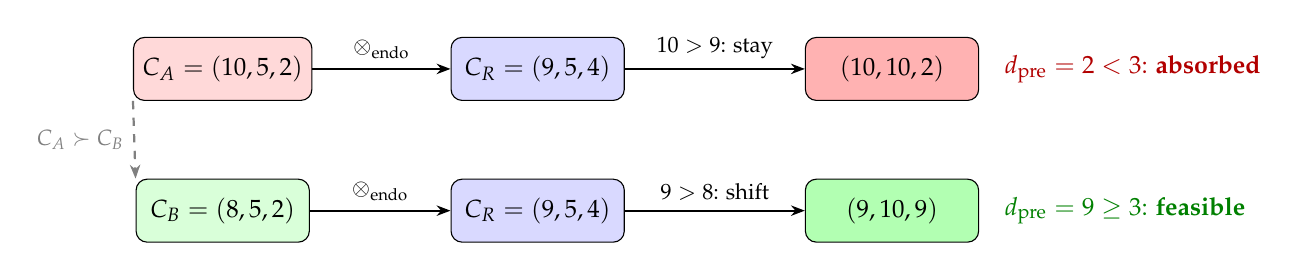
\begin{tikzpicture}[
  block/.style={draw, rounded corners, minimum width=2.2cm,
    minimum height=0.8cm, font=\small},
  arr/.style={-{Stealth[length=5pt]}, thick},
  >=Stealth
]
  % C_A path (top)
  \node[block, fill=red!15] (CA) at (0, 1.2) {$C_A = (10,5,2)$};
  \node[block, fill=blue!15] (CR1) at (4, 1.2) {$C_R = (9,5,4)$};
  \node[block, fill=red!30] (res1) at (8.5, 1.2) {$(10,10,2)$};
  \draw[arr] (CA) -- node[above, font=\footnotesize] {$\opendo$} (CR1);
  \draw[arr] (CR1) -- node[above, font=\footnotesize]
    {$10 > 9$: stay} (res1);
  \node[right=0.2cm of res1, font=\small, red!70!black]
    {$\dpre = 2 < 3$: \textbf{absorbed}};

  % C_B path (bottom)
  \node[block, fill=green!15] (CB) at (0, -0.6) {$C_B = (8,5,2)$};
  \node[block, fill=blue!15] (CR2) at (4, -0.6) {$C_R = (9,5,4)$};
  \node[block, fill=green!30] (res2) at (8.5, -0.6) {$(9,10,9)$};
  \draw[arr] (CB) -- node[above, font=\footnotesize] {$\opendo$} (CR2);
  \draw[arr] (CR2) -- node[above, font=\footnotesize]
    {$9 > 8$: shift} (res2);
  \node[right=0.2cm of res2, font=\small, green!50!black]
    {$\dpre = 9 \ge 3$: \textbf{feasible}};

  % Pareto arrow
  \draw[arr, dashed, gray] (CA.south west) -- (CB.north west)
    node[midway, left, font=\footnotesize, gray] {$C_A \succ C_B$};
\end{tikzpicture}
\caption{Monotonicity obstruction ($k = 3$, $N = 4$).  Despite
  $C_A$ Pareto-dominating $C_B$, composition with the same suffix $C_R$
  yields absorption for $C_A$ but feasibility for $C_B$.  The heavier
  pivot in $C_A$ prevents the rightward shift that would promote
  predecessors.}
\label{fig:monotonicity}
\end{figure}

% ── 3.2 L2: The Tropical Vector ──────────────────────────────
\subsection{L2: The Tropical Vector}\label{subsec:l2}

The monotonicity obstruction (\cref{thm:monotonicity-obstruction})
shows that L1 cannot support safe parallel pruning of pivot
hypotheses.  We resolve this by lifting to the tropical vector.

\begin{definition}[Tropical context]\label{def:tropical-context}
A \textbf{tropical context} is a pair
$\Ctrop = (W, \dtotal)$ where:
\begin{enumerate}[label=(\roman*),nosep]
  \item $W \in (\R \cup \{-\infty\})^{k+1}$ is the \textbf{weight
    vector}.  The entry $W[j]$ for $j = 0, 1, \ldots, k$ is the
    maximum weight among all focal events in the block with \emph{at
    least} $j$ preceding non-focal events.  The vector is
    non-increasing: $W[0] \ge W[1] \ge \cdots \ge W[k]$.
  \item $\dtotal \in \N$ is the total development capacity.
\end{enumerate}
\end{definition}

\begin{remark}[Cumulative, not exact]\label{rem:cumulative}
The definition of $W[j]$ uses ``at least $j$'' predecessors, not
``exactly $j$.''  This is essential: the cumulative definition
guarantees the non-increasing property $W[0] \ge W[1] \ge \cdots \ge
W[k]$, which in turn is required for the monotonicity proof
(\cref{thm:tropical-resolution}).  An exact-$j$ definition would break
the non-increasing property and the entire L2 theory.
\end{remark}

\begin{definition}[Tropical composition $\optrop$]
\label{def:tropical-composition}
Let $T_A = (W_A, d_A)$ and $T_B = (W_B, d_B)$.  Their tropical
composition is $T_A \optrop T_B = (W_{\mathrm{result}}, d_A + d_B)$
where:
\begin{equation}\label{eq:shift-and-max}
  W_{\mathrm{result}}[j]
  = \max\!\bigl(W_A[j],\; W_B[\max(0,\, j - d_A)]\bigr),
  \quad j = 0, 1, \ldots, k.
\end{equation}
The rule says: to be eligible at budget $j$ in the combined block, a
$B$-event needs $\ge \max(0, j - d_A)$ internal predecessors (the
remaining predecessors come from $A$'s $d_A$ non-focal events).
\end{definition}

\begin{remark}[Non-increasing preservation]\label{rem:non-increasing}
Since $\max(0, j - d_A)$ is non-decreasing in $j$ and $W_B$ is
non-increasing, $W_B[\max(0, j - d_A)]$ is non-increasing in $j$.  The
pointwise $\max$ of two non-increasing sequences is non-increasing, so
$W_{\mathrm{result}}$ is non-increasing whenever $W_A$ and $W_B$ are.
\end{remark}

\begin{theorem}[Tropical resolution]\label{thm:tropical-resolution}
The tropical composition $\optrop$ is associative and monotone in both
arguments under Pareto dominance (pointwise comparison of $W$ and
comparison of $\dtotal$).
\end{theorem}

\begin{proof}
\emph{Associativity.}  The $\dtotal$ component is additive.
For the weight vector, $(T_A \optrop T_B) \optrop T_C$ at slot $j$:
\begin{align*}
  &\max\!\Bigl(\max\bigl(W_A[j],\; W_B[\max(0, j{-}d_A)]\bigr),\;
    W_C\bigl[\max\bigl(0,\, j - d_A - d_B\bigr)\bigr]\Bigr)\\
  &= \max\!\bigl(W_A[j],\; W_B[\max(0, j{-}d_A)],\;
    W_C[\max(0, j{-}d_A{-}d_B)]\bigr).
\end{align*}
And $T_A \optrop (T_B \optrop T_C)$ at slot $j$, writing
$j' = \max(0, j - d_A)$:
\begin{align*}
  &\max\!\bigl(W_A[j],\;
    \max(W_B[j'],\; W_C[\max(0, j'{-}d_B)])\bigr)\\
  &= \max\!\bigl(W_A[j],\; W_B[\max(0, j{-}d_A)],\;
    W_C[\max(0, \max(0, j{-}d_A){-}d_B)]\bigr).
\end{align*}
These agree because $\max(0, \max(0, j{-}d_A) - d_B)
= \max(0, j - d_A - d_B)$ (both clamp at $0$).

\emph{Right-monotonicity.}  Assume $T_A \succeq T_B$, i.e.,
$W_A[j] \ge W_B[j]$ for all $j$ and $d_A \ge d_B$.  Fix $T_R$.
\[
  (T_A \optrop T_R)[j] = \max\bigl(W_A[j],\; W_R[\max(0, j{-}d_A)]\bigr).
\]
First term: $W_A[j] \ge W_B[j]$.
Second term: $d_A \ge d_B$ implies $\max(0, j{-}d_A) \le \max(0,
j{-}d_B)$, so $W_R[\max(0, j{-}d_A)] \ge W_R[\max(0, j{-}d_B)]$
(since $W_R$ is non-increasing).  Therefore
$(T_A \optrop T_R)[j] \ge (T_B \optrop T_R)[j]$.

Left-monotonicity is analogous.
\end{proof}

\begin{remark}[Recovering L1 from L2]\label{rem:recovering-l1}
Given $\Ctrop = (W, \dtotal)$, the L1 summary is
$\wstar = \max_{0 \le j \le k} W[j] = W[0]$ (by the non-increasing
property) and $\dpre = \max\{j : W[j] = W[0]\}$, the highest slot
achieving the maximum.  L2 is strictly richer: it records feasibility
at every threshold simultaneously.
\end{remark}

% ── 3.3 L3: The Frontier Semiring ────────────────────────────
\subsection{L3: The Frontier Semiring}\label{subsec:l3}

\begin{definition}[Frontier semiring]\label{def:frontier}
The \textbf{L3 frontier} is the set $\Ant(\Ctrop)$ of finite
antichains in the Pareto order on tropical contexts.  The semiring
operations are:
\begin{align*}
  A \oplus B &= \mathrm{cl}(A \cup B),\\
  A \otimes B &= \mathrm{cl}\!\bigl(\{a \optrop b : a \in A, b \in B\}\bigr),
\end{align*}
where $\mathrm{cl}$ denotes Pareto closure (removing dominated
elements).  This yields an idempotent semiring that supports $O(\log n)$
parallel tree reductions.
\end{definition}

The three levels form a refinement hierarchy:
\[
  \text{L1 (scalar)} \hookrightarrow
  \text{L2 (tropical vector)} \hookrightarrow
  \text{L3 (frontier semiring)}.
\]
L1 is $O(1)$ per event but admits absorption.  L2 is $O(k)$ per event
and is monotone.  L3 is $O(|\text{antichain}|)$ per event and
maintains multiple hypotheses.

% ── Algebraic Tower Figure ────────────────────────────────────
\begin{figure}[t]
\centering
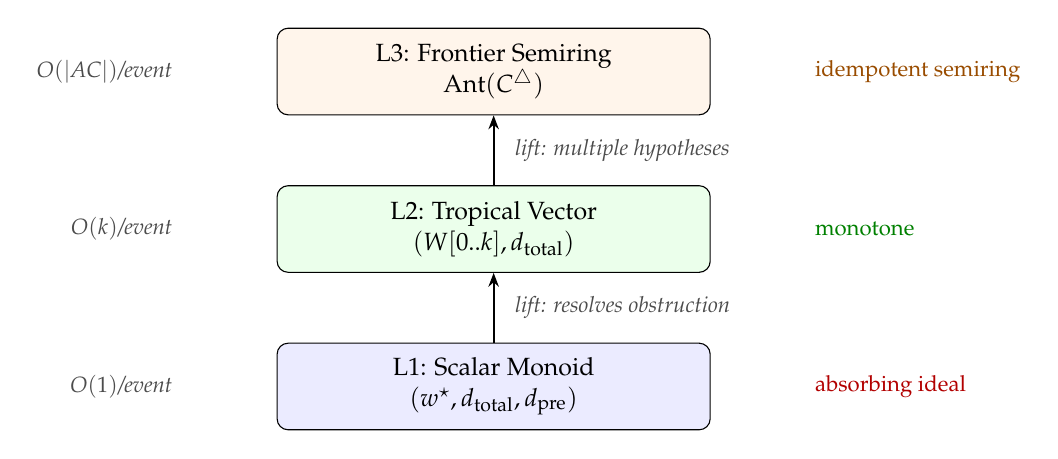
\begin{tikzpicture}[
  level/.style={draw, rounded corners, minimum width=5.5cm,
    minimum height=1.1cm, align=center, font=\small},
  arr/.style={-{Stealth[length=5pt]}, thick},
  lbl/.style={font=\footnotesize\itshape, text=black!70},
]
  \node[level, fill=blue!8] (l1) at (0,0)
    {L1: Scalar Monoid\\$(\wstar, \dtotal, \dpre)$};
  \node[level, fill=green!8] (l2) at (0,2)
    {L2: Tropical Vector\\$(W[0..k], \dtotal)$};
  \node[level, fill=orange!8] (l3) at (0,4)
    {L3: Frontier Semiring\\$\Ant(\Ctrop)$};

  \draw[arr] (l1) -- (l2)
    node[midway, right=4pt, lbl] {lift: resolves obstruction};
  \draw[arr] (l2) -- (l3)
    node[midway, right=4pt, lbl] {lift: multiple hypotheses};

  \node[lbl, left=1.2cm of l1] {$O(1)$/event};
  \node[lbl, left=1.2cm of l2] {$O(k)$/event};
  \node[lbl, left=1.2cm of l3] {$O(|\text{AC}|)$/event};

  \node[font=\footnotesize, text=red!70!black, right=1.2cm of l1]
    {absorbing ideal};
  \node[font=\footnotesize, text=green!50!black, right=1.2cm of l2]
    {monotone};
  \node[font=\footnotesize, text=orange!60!black, right=1.2cm of l3]
    {idempotent semiring};
\end{tikzpicture}
\caption{The algebraic tower.  Each level refines the one below,
  trading computational cost for richer structural guarantees.  L2 is
  the minimal monotone level (\cref{thm:myhill-nerode}).}
\label{fig:tower}
\end{figure}

% ══════════════════════════════════════════════════════════════
\section{Tropical Matrix Equivalence}\label{sec:tropical-matrix}
% ══════════════════════════════════════════════════════════════

We now show that L2 composition is isomorphic to tropical matrix
multiplication, connecting the endogenous-pivot algebra to the
classical theory of max-plus linear systems
\cite{baccelli1992synchronization}.

\begin{definition}[Tropical semiring]\label{def:tropical-semiring}
The \textbf{tropical semiring} (max-plus) is
$\Tmax = (\R \cup \{-\infty\}, \oplus, \odot)$ where $a \oplus b =
\max(a,b)$ and $a \odot b = a + b$, with additive identity $-\infty$
and multiplicative identity $0$.
\end{definition}

\begin{definition}[Tropical matrix encoding]\label{def:tropical-matrix}
Given a tropical context $T_A = (W_A, d_A)$ with threshold $k$,
define the $(k{+}2) \times (k{+}2)$ tropical matrix $M_A$ over
$\Tmax$ as follows.  Index rows and columns by $\{0, 1, \ldots, k, \star\}$
where $\star$ denotes the homogeneous coordinate.

\begin{enumerate}[label=(\roman*),nosep]
  \item \textbf{Shift block} (rows and columns $0, \ldots, k$):
    For $0 \le i, j \le k$,
    \[
      (M_A)_{ij} = \begin{cases}
        0 & \text{if } j = \max(0,\, i - d_A),\\
        -\infty & \text{otherwise}.
      \end{cases}
    \]
    Row $i$ has a single active entry at column $\max(0, i - d_A)$:
    the predecessor budget that a $B$-event would need internally to
    reach total budget $i$ given $d_A$ predecessors from~$A$.

  \item \textbf{Weight column} (column $\star$, rows $0, \ldots, k$):
    $(M_A)_{j,\star} = W_A[j]$ for $0 \le j \le k$.

  \item \textbf{Homogeneous row and entry}:
    $(M_A)_{\star,j} = -\infty$ for $0 \le j \le k$, and
    $(M_A)_{\star,\star} = 0$.
\end{enumerate}
\end{definition}

% ── Matrix Structure Figure ───────────────────────────────────
\begin{figure}[t]
\centering
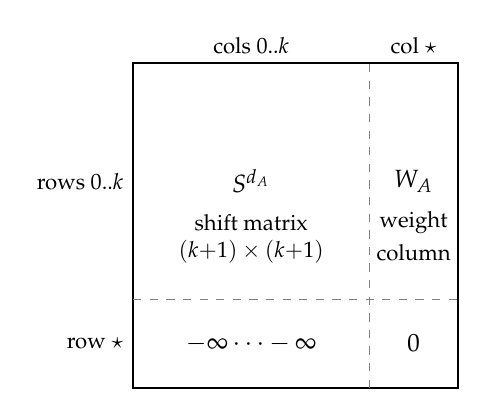
\begin{tikzpicture}[scale=0.75, font=\small]
  \draw[thick] (0,0) rectangle (5.5,5.5);
  % Block labels
  \draw[dashed, gray] (4,0) -- (4,5.5);
  \draw[dashed, gray] (0,1.5) -- (5.5,1.5);
  % Labels
  \node at (2,3.5) {$S^{d_A}$};
  \node[font=\footnotesize] at (2,2.8) {shift matrix};
  \node[font=\footnotesize] at (2,2.3) {$(k{+}1) \times (k{+}1)$};
  \node at (4.75,3.5) {$W_A$};
  \node[font=\footnotesize] at (4.75,2.8) {weight};
  \node[font=\footnotesize] at (4.75,2.3) {column};
  \node at (2,0.75) {$-\infty \cdots -\infty$};
  \node at (4.75,0.75) {$0$};
  % Row/column labels
  \node[font=\footnotesize, left] at (0,3.5) {rows $0..k$};
  \node[font=\footnotesize, left] at (0,0.75) {row $\star$};
  \node[font=\footnotesize, above] at (2,5.5) {cols $0..k$};
  \node[font=\footnotesize, above] at (4.75,5.5) {col $\star$};
\end{tikzpicture}
\caption{Structure of the $(k{+}2) \times (k{+}2)$ tropical matrix
  $M_A$.  The shift block encodes the predecessor-count shift by
  $d_A$.  The weight column records the feasibility frontier.  The
  homogeneous coordinate preserves $W$ values under multiplication.}
\label{fig:matrix}
\end{figure}

\begin{theorem}[Tropical matrix equivalence]\label{thm:tropical-matrix}
For any tropical contexts $T_A = (W_A, d_A)$ and $T_B = (W_B, d_B)$
with the same threshold $k$, the tropical matrix product satisfies
\[
  M_{T_A \optrop T_B} = M_A \otimes_{\Tmax} M_B,
\]
where $\otimes_{\Tmax}$ denotes tropical (max-plus) matrix
multiplication.

Consequently, the stream reduction
$T_{\mathrm{out}} = T_{e_1} \optrop T_{e_2} \optrop \cdots \optrop
T_{e_n}$ is computed by the tropical matrix product
$M_{e_1} \otimes_{\Tmax} M_{e_2} \otimes_{\Tmax} \cdots
\otimes_{\Tmax} M_{e_n}$, which admits $O(\log n)$ parallel depth via
repeated squaring, with each multiplication costing $O(k^2)$ tropical
operations.
\end{theorem}

\begin{proof}
We verify that the matrix product $M_A \otimes_{\Tmax} M_B$ reproduces
the composition rule of \cref{def:tropical-composition}.

\emph{Shift block.}  For rows and columns in $\{0, \ldots, k\}$:
\[
  (M_A \otimes M_B)_{ij}
  = \bigoplus_{\ell=0}^{k} (M_A)_{i\ell} \odot (M_B)_{\ell j}
  \oplus (M_A)_{i,\star} \odot (M_B)_{\star,j}.
\]
The last term vanishes since $(M_B)_{\star,j} = -\infty$ for
$j \le k$.  In the sum, $(M_A)_{i\ell} \ne -\infty$ only when
$\ell = \max(0, i - d_A)$, and $(M_B)_{\ell j} \ne -\infty$ only when
$j = \max(0, \ell - d_B)$.  So the product entry is $0$ exactly when
$j = \max(0, \max(0, i - d_A) - d_B) = \max(0, i - d_A - d_B)$,
which matches the shift block of $M_{T_A \optrop T_B}$ (combined shift
$d_A + d_B$).

\emph{Weight column.}  For row $j \in \{0, \ldots, k\}$ and column
$\star$:
\begin{align*}
  (M_A \otimes M_B)_{j,\star}
  &= \bigoplus_{\ell=0}^{k} (M_A)_{j\ell} \odot (M_B)_{\ell,\star}
     \;\oplus\; (M_A)_{j,\star} \odot (M_B)_{\star,\star}\\
  &= (M_B)_{\max(0,j-d_A),\star}
     \;\oplus\; (M_A)_{j,\star} \odot 0\\
  &= \max\!\bigl(W_B[\max(0, j - d_A)],\; W_A[j]\bigr),
\end{align*}
which is exactly the composition rule \eqref{eq:shift-and-max}.

\emph{Homogeneous entries.}  $(M_A \otimes M_B)_{\star,\star} =
(M_A)_{\star,\star} \odot (M_B)_{\star,\star} = 0 + 0 = 0$.  The
remaining entries $(M_A \otimes M_B)_{\star,j} = -\infty$ for $j \le k$
since $(M_A)_{\star,\ell} = -\infty$ for all $\ell \le k$.

All blocks match.  The isomorphism follows.
\end{proof}

\begin{example}[Tropical matrix multiplication at $k = 2$]
\label{ex:matrix-k2}
Let $T_A = ([3, 3, -\infty],\; 1)$ (one non-focal event, one focal
event of weight~$3$ with $1$~predecessor) and $T_B = ([5, -\infty,
-\infty],\; 2)$ (two non-focal events, one focal event of weight~$5$
with $0$~predecessors).  Their $4 \times 4$ matrices (under the
corrected encoding with $\max(0, i - d)$):
\[
  M_A = \begin{pmatrix}
    0 & -\infty & -\infty & 3 \\
    0 & -\infty & -\infty & 3 \\
    -\infty & 0 & -\infty & -\infty \\
    -\infty & -\infty & -\infty & 0
  \end{pmatrix},
  \quad
  M_B = \begin{pmatrix}
    0 & -\infty & -\infty & 5 \\
    0 & -\infty & -\infty & -\infty \\
    0 & -\infty & -\infty & -\infty \\
    -\infty & -\infty & -\infty & 0
  \end{pmatrix}.
\]
In $M_A$ ($d_A = 1$): row $i$ has a~$0$ at column $\max(0, i - 1)$.
So rows $0$ and $1$ both activate column~$0$; row $2$ activates
column~$1$.  In $M_B$ ($d_B = 2$): rows $0$, $1$, $2$ all activate
column~$0$.

\smallskip
The tropical product $M_A \otimes_{\Tmax} M_B$:
\begin{itemize}[nosep]
  \item \emph{Shift block:} Row~$0$ routes through $\ell = 0$ in $A$,
    then row~$0$ in $B$ activates column~$0$.  Product shift:
    $\max(0, 0 - 1 - 2) = 0$.  Active at $(0,0)$.
  \item \emph{Weight column, row~$0$:}
    $\max(W_B[\max(0, 0{-}1)],\; W_A[0]) = \max(W_B[0], 3) =
    \max(5, 3) = 5$.
  \item \emph{Weight column, row~$1$:}
    $\max(W_B[\max(0, 1{-}1)],\; W_A[1]) = \max(W_B[0], 3) =
    \max(5, 3) = 5$.
  \item \emph{Weight column, row~$2$:}
    $\max(W_B[\max(0, 2{-}1)],\; W_A[2]) = \max(W_B[1], -\infty) =
    -\infty$.
\end{itemize}
Result: $T_{AB} = ([5, 5, -\infty],\; 3)$.  Non-increasing, correct:
$B$'s weight-$5$ focal event has $0$ internal predecessors plus $d_A =
1$ from $A$, so it qualifies at budgets $0$ and $1$.  $A$'s weight-$3$
focal event is dominated at both slots.
\end{example}

\begin{corollary}\label{cor:parallel}
The tropical context of an $n$-event stream can be computed in
$O(k^2 \log n)$ parallel time (or $O(nk)$ sequential time), where each
matrix multiplication costs $O(k^2)$ tropical operations.
\end{corollary}

% ══════════════════════════════════════════════════════════════
\section{Necessity: L2 is Optimal}\label{sec:necessity}
% ══════════════════════════════════════════════════════════════

We now prove that no summary with fewer than $k+1$ components can
replace L2.  The argument adapts the Myhill--Nerode theorem
\cite{hopcroft1979introduction} from automata theory to tropical
summaries.

\begin{definition}[Valid summary]\label{def:valid-summary}
A \textbf{valid summary} for the endogenous-pivot extraction problem
with prefix requirement $k$ is a triple $(\mathcal{S}, \otimes_S,
\pi)$ where:
\begin{enumerate}[label=(\roman*),nosep]
  \item $\mathcal{S}$ is a set of summary states;
  \item $\otimes_S \colon \mathcal{S} \times \mathcal{S} \to
    \mathcal{S}$ is an associative binary operation;
  \item $\pi \colon \mathcal{S} \to \{0,1\}$ is a feasibility
    predicate;
\end{enumerate}
such that: (a) every event block maps to a unique summary state via a
homomorphism $h$; (b) $\pi(h(\text{block})) = 1$ iff the block is
feasible at threshold~$k$; and (c) $h(A \cdot B) = h(A) \otimes_S
h(B)$ (composition respects concatenation).

A valid summary is \textbf{dominance-monotone} if it admits a partial
order $\preceq$ on $\mathcal{S}$ such that (i) $s \preceq s'$ implies
$s \otimes_S r \preceq s' \otimes_S r$ and $r \otimes_S s \preceq r
\otimes_S s'$ for all $r$, and (ii) $\pi$ is upward closed with
respect to $\preceq$.
\end{definition}

\begin{theorem}[Myhill--Nerode necessity]\label{thm:myhill-nerode}
For singleton path-independent endogenous-pivot systems with prefix
requirement $k \ge 1$:
\begin{enumerate}[label=(\alph*)]
  \item Any valid, dominance-monotone summary requires
    $|\mathcal{S}| \ge k + 1$ distinct states (equivalently, the
    summary must carry at least $\Omega(k)$ information).
  \item L2 achieves this bound with exactly $k+1$ weight-vector
    entries plus one integer $\dtotal$.
\end{enumerate}
\end{theorem}

\begin{proof}
\emph{Part~(a): Lower bound via separating suffixes.}

Define the \textbf{syntactic right-congruence} $\sim$ on summary
states: $s_1 \sim s_2$ iff for every suffix stream $X$,
$\pi(s_1 \otimes_S h(X)) = \pi(s_2 \otimes_S h(X))$.  By the
Myhill--Nerode theorem, the number of equivalence classes of $\sim$
equals the minimum number of states in any valid summary.

We exhibit $k+1$ pairwise inequivalent L2 states.  For
$j = 0, 1, \ldots, k$, define $T_j$ as the tropical context of a
stream consisting of $j$ non-focal events followed by one focal event
of weight~$0$.  Then $T_j = (W_j, d_j)$ where $d_j = j$ and:
\[
  W_j[\ell] = \begin{cases}
    0 & \text{if } \ell \le j,\\
    -\infty & \text{if } \ell > j.
  \end{cases}
\]
(The focal event has at least $\ell$ predecessors for all $\ell \le j$,
using the cumulative definition of $W$.)

\emph{Claim:} $T_i \not\sim T_j$ for $0 \le i < j \le k$.

\emph{Separating suffix construction.}
Given $i < j$, construct a suffix block $X$ consisting of $k - i - 1$
non-focal events followed by one focal event of weight $\beta = -1$.
The suffix's tropical context is $T_X = (W_X,\; k{-}i{-}1)$ with
$W_X[\ell] = -1$ for $\ell \le k - i - 1$ and $-\infty$ otherwise.

\emph{Composing $T_i \optrop T_X$:}  The left block has $d_i = i$.
A suffix focal event at slot $\ell'$ shifts to result slot
$\min(\ell' + i, k)$.  The highest occupied suffix slot is
$\ell' = k - i - 1$, which shifts to $\min(k - 1, k) = k - 1$.
No suffix slot reaches $k$ with finite weight (slot $k - i$ would be
needed, but $W_X[k-i] = -\infty$).  Meanwhile, $T_i$'s own
contribution at slot $k$ is $W_i[k] = -\infty$ since $k > i$.
Therefore $W_{\mathrm{result}}[k] = -\infty$: the composition is
\textbf{infeasible}.

\emph{Composing $T_j \optrop T_X$ (with $j \ge i + 1$):}  The left
block has $d_j = j$.  The suffix focal event at slot $k - i - 1$
shifts to $\min(k - i - 1 + j, k)$.  Since $j \ge i + 1$, this equals
$\min(k, k) = k$, contributing weight $\beta = -1$ to slot $k$.
If $j < k$: $W_j[k] = -\infty$, but the suffix contributes $-1$, so
$W_{\mathrm{result}}[k] = -1 > -\infty$.
If $j = k$: $W_j[k] = 0$, so $W_{\mathrm{result}}[k] \ge 0$.
In both cases: \textbf{feasible}.

The suffix $X$ thus separates $T_i$ from $T_j$: composition with $X$
is infeasible for $T_i$ but feasible for $T_j$.  Since this works for
all $0 \le i < j \le k$, the $k+1$ states $T_0, \ldots, T_k$ are
pairwise inequivalent under the syntactic right-congruence, requiring
at least $k + 1$ equivalence classes.

\begin{example}[Separating suffixes at $k = 3$]\label{ex:myhill-nerode-k3}
The four inequivalent states are:
\begin{align*}
  T_0 &= \bigl([0, -\infty, -\infty, -\infty],\; 0\bigr),\\
  T_1 &= \bigl([0, 0, -\infty, -\infty],\; 1\bigr),\\
  T_2 &= \bigl([0, 0, 0, -\infty],\; 2\bigr),\\
  T_3 &= \bigl([0, 0, 0, 0],\; 3\bigr).
\end{align*}
To separate $T_1$ from $T_2$: construct a suffix of $3 - 1 - 1 = 1$
non-focal event plus one focal event of weight $-1$.  The suffix
context is $T_X = ([-1, -1, -\infty, -\infty],\; 1)$.
\begin{itemize}[nosep]
  \item $T_1 \optrop T_X$: suffix slot $1$ shifts to
    $\min(1 + 1, 3) = 2$.  Slot $3$ gets $-\infty$ from both.
    \textbf{Infeasible.}
  \item $T_2 \optrop T_X$: suffix slot $1$ shifts to
    $\min(1 + 2, 3) = 3$, contributing $-1$.  Slot $3$ is alive.
    \textbf{Feasible.}
\end{itemize}
\end{example}

\emph{Part~(b): L2 achieves the bound.}

L2 uses $k+1$ weight-vector entries plus $\dtotal$, giving $k+2$ total
components.  Every valid summary must encode at least $k+1$ distinct
feasibility classes (from part~(a)).  L2 achieves this minimum while
also being associative and dominance-monotone
(\cref{thm:tropical-resolution}).

We conjecture that L2 is, moreover, the \emph{initial object} in the
category of valid summaries: every valid, dominance-monotone summary
$(\mathcal{S}, \otimes_S, \pi)$ factors through L2 via a natural map
$f \colon \mathcal{S} \to (\R \cup \{-\infty\})^{k+1} \times \N$
extracting the maximum focal weight achievable with at least $j$
predecessors for each $j$.  The lower bound (part~(a)) and
optimality (part~(b)) do not depend on this conjecture.
\end{proof}

% ══════════════════════════════════════════════════════════════
\section{The Record-Gap Spectrum}\label{sec:record-gap}
% ══════════════════════════════════════════════════════════════

We now derive the exact Poisson intensities governing non-focal gap
sizes in streaming event sequences.  This provides the asymptotic
baseline for trap rates under pure streaming (no compression).

\begin{definition}[Focal-mask model]\label{def:focal-mask}
In the \textbf{focal-mask model}, each event in a stream is
independently focal with probability $p \in (0,1)$.  Conditional on
being focal, events have i.i.d.\ continuous weight distributions.
Non-focal events contribute to development capacity but cannot serve as
pivots.
\end{definition}

\begin{definition}[Record and record gap]\label{def:record-gap}
A \textbf{focal record} is a focal event whose weight exceeds all
previous focal events.  A \textbf{record gap} of size $g$ (measured in
non-focal events) is a run of $g$ consecutive non-focal events between
two consecutive focal records.  The \textbf{minimum gap} of a stream is
$\min_g(\text{record gap})$; feasibility at threshold $k$ requires
minimum gap $\ge k$.
\end{definition}

\begin{theorem}[Record-gap spectrum]\label{thm:record-gap}
Under the focal-mask model with parameter $p$, the number $N_g$ of
record gaps of non-focal size $g$ is asymptotically Poisson with
intensity:
\begin{equation}\label{eq:lambda-g}
  \lambda_g(p) = \frac{1 - (1-p)^g}{g}, \quad g \ge 1,
  \qquad
  \lambda_0(p) = -\ln(1-p).
\end{equation}
The gap counts $\{N_g\}_{g \ge 0}$ are asymptotically independent.
The probability that all record gaps have non-focal size $\ge k$
converges to:
\begin{equation}\label{eq:survival}
  \Pr(\min\text{-gap} \ge k) \to \exp\!\Bigl(-\sum_{g=0}^{k-1}
  \lambda_g(p)\Bigr) = \exp(-\Lambda_k(p)).
\end{equation}
The gap spectrum belongs to the Ewens$(\theta = 1)$ universality class:
$\lambda_g(p) = \int_0^{-\ln(1-p)} e^{-gy}\, dy$, matching the
Ewens$(\theta=1)$ truncated L\'evy measure via Chinese Restaurant
Process coupling with geometric subordination.
\end{theorem}

\begin{proof}
The proof proceeds in five steps.

\textbf{Step~A: Classical record-gap spectrum on the focal
subsequence.}  Extract the subsequence of focal events.  By the theory
of records for i.i.d.\ continuous random variables
\cite{nevzorov2001records,arnold1998records,renyi1962theorie}, the
number of focal gaps of focal-length $j$ (i.e., $j$ non-record focal
events between consecutive records) is asymptotically Poisson with
intensity $1/j$, and these counts are asymptotically independent.

\textbf{Step~B: Non-focal gap distribution.}  Between two consecutive
focal events separated by focal-length $j$ (meaning $j$ focal events
lie between the two records in the full sequence), the number of
non-focal events interspersed is negative-binomially distributed.  Each
inter-focal slot independently contains a geometric number of non-focal
events.  Precisely, if $G$ is the total non-focal count in a
focal-length-$j$ gap, then:
\[
  G \mid j \;\sim\; \mathrm{NegBin}(j, p).
\]
This holds because each of the $j$ inter-record focal events is
preceded by a geometric$(p)$ run of non-focal events.

\textbf{Step~C: Poisson marking.}  The number of focal gaps of
focal-length $j$ is $M_j \sim \mathrm{Poisson}(1/j)$.  Each such gap
independently produces a non-focal gap $G \sim \mathrm{NegBin}(j,p)$.
The total number $N_g$ of gaps with non-focal size exactly $g$ is:
\[
  N_g \sim \mathrm{Poisson}\!\Bigl(\sum_{j=1}^{\infty}
  \frac{1}{j} \Pr(\mathrm{NegBin}(j,p) = g)\Bigr).
\]
Independence across $g$ follows from the Poisson coloring theorem.

\textbf{Step~D: Generating function collapse.}  Define:
\[
  S_g(x) = \sum_{j=1}^{\infty} \frac{1}{j} \binom{g+j-1}{g} x^j.
\]
The intensity we seek is $\lambda_g(p) = (1-p)^g \cdot S_g(p)$.
Differentiate term by term:
\[
  S_g'(x) = \sum_{j=1}^{\infty} \binom{g+j-1}{g} x^{j-1}
  = \sum_{m=0}^{\infty} \binom{g+m}{g} x^m
  = \frac{1}{(1-x)^{g+1}},
\]
where the last equality is the generating function for multiset
coefficients.  Integrate from $0$ to $p$:
\[
  S_g(p) = \int_0^p \frac{dx}{(1-x)^{g+1}}
  = \frac{(1-p)^{-g} - 1}{g}.
\]
Multiply by $(1-p)^g$:
\begin{equation}\label{eq:lambda-derivation}
  \lambda_g(p) = (1-p)^g \cdot \frac{(1-p)^{-g} - 1}{g}
  = \frac{1 - (1-p)^g}{g}. \qquad\checkmark
\end{equation}

\textbf{Step~E: Independence and CRP coupling.}  Independence of the
$\{N_g\}$ counts follows from the Poisson coloring theorem applied in
Step~C, with rigorous control via Chen--Stein second-moment bounds
\cite{arratia2003logarithmic}.

For the CRP coupling, observe that:
\[
  \lambda_g(p) = \int_0^{-\ln(1-p)} e^{-gy}\, dy
  = \int_0^a e^{-gy}\, dy,
\]
where $a = -\ln(1-p)$.  The measure $e^{-gy}\, dy$ on $(0,\infty)$ is
exactly the L\'evy measure of a Gamma subordinator, which governs table
sizes in the Chinese Restaurant Process with parameter $\theta = 1$
\cite{pitman2006combinatorial}.  The truncation at $a = -\ln(1-p)$
arises from the geometric subordination (masking with retention
probability $1-p$).
\end{proof}

\begin{remark}[Sanity checks]\label{rem:sanity}
The formula $\lambda_g(p) = [1-(1-p)^g]/g$ passes several checks:
\begin{enumerate}[label=(\roman*),nosep]
  \item $k = 1$: $\Pr(\min\text{-gap} \ge 1) \to
    \exp(-\lambda_0) = 1-p$.  Correct: the only failing configuration
    is two consecutive focal records with no intervening non-focal
    event, which happens when the first event is focal and a record.
  \item $k = 2$: $\Pr(\min\text{-gap} \ge 2) \to (1-p) \cdot e^{-p}$.
  \item Large $g$: $\lambda_g(p) \to 1/g$, recovering the classical
    harmonic record spectrum (no masking).
  \item Small $p$: $\Lambda_k(p) \approx kp$, giving
    $\Pr(\min\text{-gap} \ge k) \approx e^{-kp}$.
\end{enumerate}
At canonical parameters $p = 0.367$, $k = 3$:
$\Lambda_3 \approx 1.1239$ and
$S_\infty = \exp(-\Lambda_3) \approx 0.3250$.
\end{remark}

\begin{figure}[t]
\centering
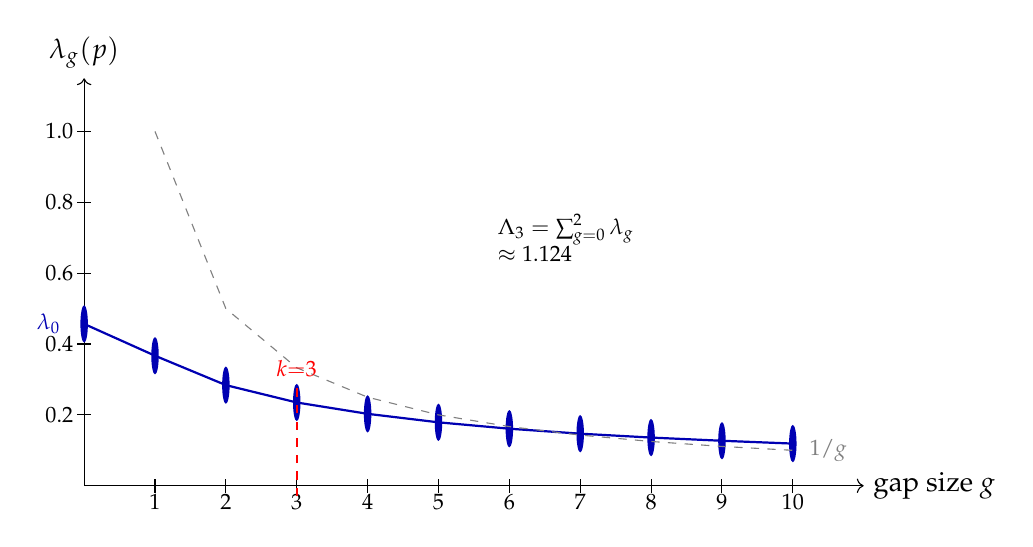
\begin{tikzpicture}[xscale=0.9, yscale=4.5]
  % Axes
  \draw[->] (0,0) -- (11,0) node[right] {gap size $g$};
  \draw[->] (0,0) -- (0,1.15) node[above] {$\lambda_g(p)$};

  % Y-axis ticks
  \foreach \y/\lab in {0.2/0.2, 0.4/0.4, 0.6/0.6, 0.8/0.8, 1.0/1.0} {
    \draw (-0.1, \y) -- (0.1, \y) node[left=3pt, font=\footnotesize] {\lab};
  }
  % X-axis ticks
  \foreach \x in {1,...,10} {
    \draw (\x, -0.02) -- (\x, 0.02)
      node[below=2pt, font=\footnotesize] {\x};
  }

  % lambda_0 = -ln(1-p) ≈ 0.4567 (plotted at g=0)
  \fill[blue!70!black] (0, 0.4567) circle (1.5pt);
  \node[left=5pt, font=\footnotesize, blue!70!black] at (0, 0.4567) {$\lambda_0$};

  % lambda_g(p) = [1-(1-p)^g]/g at p = 0.367
  % g=1: 0.367, g=2: 0.284, g=3: 0.235, g=4: 0.203,
  % g=5: 0.179, g=6: 0.161, g=7: 0.147, g=8: 0.136,
  % g=9: 0.127, g=10: 0.119
  \fill[blue!70!black] (1, 0.367) circle (1.5pt);
  \fill[blue!70!black] (2, 0.284) circle (1.5pt);
  \fill[blue!70!black] (3, 0.235) circle (1.5pt);
  \fill[blue!70!black] (4, 0.203) circle (1.5pt);
  \fill[blue!70!black] (5, 0.179) circle (1.5pt);
  \fill[blue!70!black] (6, 0.161) circle (1.5pt);
  \fill[blue!70!black] (7, 0.147) circle (1.5pt);
  \fill[blue!70!black] (8, 0.136) circle (1.5pt);
  \fill[blue!70!black] (9, 0.127) circle (1.5pt);
  \fill[blue!70!black] (10, 0.119) circle (1.5pt);

  % Connect with line
  \draw[blue!70!black, thick]
    (0, 0.4567) -- (1, 0.367) -- (2, 0.284) -- (3, 0.235) --
    (4, 0.203) -- (5, 0.179) -- (6, 0.161) -- (7, 0.147) --
    (8, 0.136) -- (9, 0.127) -- (10, 0.119);

  % Classical 1/g reference (dashed)
  \draw[gray, dashed, thin]
    (1, 1.0) -- (2, 0.5) -- (3, 0.333) -- (4, 0.25) --
    (5, 0.2) -- (6, 0.167) -- (7, 0.143) -- (8, 0.125) --
    (9, 0.111) -- (10, 0.1);
  \node[gray, font=\footnotesize, right] at (10.1, 0.1) {$1/g$};

  % k threshold
  \draw[red, thick, dashed] (3, -0.03) -- (3, 0.28);
  \node[red, font=\footnotesize, above] at (3, 0.28) {$k{=}3$};

  % Annotation
  \node[font=\footnotesize, text width=3cm, align=left] at (7.5, 0.7)
    {$\Lambda_3 = \sum_{g=0}^{2}\lambda_g$\\$\approx 1.124$};
\end{tikzpicture}
\caption{Record-gap spectrum $\lambda_g(p)$ at $p = 0.367$ (solid
  blue) vs.\ the classical harmonic spectrum $1/g$ (dashed gray).
  The focal-mask model suppresses short gaps: $\lambda_g(p) < 1/g$ for
  all $g$.  Feasibility at $k = 3$ requires all gaps $\ge 3$; the
  cumulative intensity $\Lambda_3 \approx 1.124$ gives asymptotic
  survival $S_\infty = e^{-\Lambda_3} \approx 0.325$.}
\label{fig:record-gap}
\end{figure}

% ══════════════════════════════════════════════════════════════
\section{Dynamics Under Compression}\label{sec:dynamics}
% ══════════════════════════════════════════════════════════════

We now analyze the compound regime where streaming pivot selection
interleaves with periodic Bernoulli thinning.  This models systems
(such as LLM context windows) where events are periodically compressed
by random deletion.

% ── 7.1 INAR(1) model ────────────────────────────────────────
\subsection{The INAR(1) Model}\label{subsec:inar}

\begin{definition}[Compound streaming model]\label{def:compound}
Fix a thinning period $T \in \N$ (number of new events per epoch),
retention probability $r \in (0,1)$, and focal probability $p$.  Each
epoch proceeds in three steps: (i)~thin all surviving events
independently with retention probability~$r$; (ii)~append $T$ new
events, each focal independently with probability~$p$; (iii)~thin the
new arrivals with the same probability~$r$ (modeling that new events
also undergo the current compression).  Let $N_n$ denote the focal
event count at the end of epoch~$n$.  Then:
\begin{equation}\label{eq:inar}
  N_{n+1} = \mathrm{Bin}(N_n, r) + \mathrm{Bin}(T, pr).
\end{equation}
The stationary focal mean is $\mu_f = Tpr/(1-r)$ and the stationary
non-focal mean is $\mu_{\mathrm{nf}} = T(1-p)r/(1-r)$.
\end{definition}

\begin{definition}[Operational semantics]\label{def:operational-semantics}
We distinguish three modes of evaluating feasibility at each epoch:
\begin{enumerate}[label=(\alph*),nosep]
  \item \textbf{Committed (L1-committed):} The system commits to the
    current $\argmax$ pivot $\tau_n$.  Predecessors undergo pure
    Bernoulli$(r)$ death; no new events can become predecessors of
    $\tau_n$ (they arrive after it temporally).  If $\dpre$ drops below
    $k$, the sequence is declared infeasible with no recovery.
  \item \textbf{L1-retry:} The system re-evaluates
    $\tau(S) = \argmax_{v \in S,\, a(v) = a^*} w(v)$ at each epoch.
    When a pivot turnover occurs (a new $\argmax$ replaces the old), the
    predecessor count resets to the new pivot's predecessor count.
    Transient infeasibility is tolerated.
  \item \textbf{L2 (full tropical):} The system maintains the
    full $W[0..k]$ vector at each epoch, tracking all possible
    predecessor budgets simultaneously.  Feasibility holds iff
    $W[k] > -\infty$.
\end{enumerate}
\end{definition}

% ── 7.2 Prefix impossibility ─────────────────────────────────
\subsection{Prefix-Constraint Impossibility}

\begin{theorem}[Prefix-constraint impossibility]
\label{thm:prefix-impossibility}
Let the greedy policy force
$e^* = \argmax_{v : a(v)=a^*} w(v)$ as turning point.  If the number
of development-eligible events before $e^*$ in the candidate pool
satisfies $\jdev < k$, then greedy produces zero valid sequences.
\end{theorem}

\begin{proof}
Greedy pre-selects $e^*$ as the turning point.  By the DFA's monotone
phase rule, no transition from \textsc{turning\_point} or
\textsc{resolution} back to \textsc{development} exists.  At most
$\jdev$ events can be classified as \textsc{development} in the
pre-pivot portion.  Since $\jdev < k$ and the grammar requires $\ge k$
\textsc{development} events before the turning point, no valid
completion exists.

Formally, this is an absorbing-state argument in the product automaton
$P = G \times \mathcal{A}$: the forced injection of $e^*$ as
\textsc{turning\_point} drives the DFA to a state from which the
acceptance condition ($\ge k$ development events) cannot be reached.
\end{proof}

% ── 7.3 Turnover universality ────────────────────────────────
\subsection{Turnover Universality}

\begin{theorem}[Turnover universality]\label{thm:turnover}
Under committed semantics with Bernoulli$(r)$ thinning ($r < 1$) and
no new predecessor arrivals to the current $\argmax$, the probability of
same-$\argmax$ recovery after $\dpre < k$ is exactly zero.
\end{theorem}

\begin{proof}
\begin{enumerate}[label=\arabic*.,nosep]
  \item Predecessors of the current pivot are events with timestamps
    strictly before the pivot.  New events arrive with later timestamps,
    so they cannot become predecessors of the existing pivot.
  \item Under Bernoulli thinning, the predecessor count evolves as
    pure death: $d_{t+1} \sim \mathrm{Bin}(d_t, r)$.
  \item This process is a non-negative supermartingale:
    $\mathbb{E}[d_{t+1} \mid d_t] = r \cdot d_t < d_t$.
  \item By the supermartingale convergence theorem, $d_t \to 0$ almost
    surely.
  \item Once $d_t < k$, no upward jumps exist (new arrivals cannot
    become predecessors), so absorption at $\dpre < k$ is permanent.
    \qedhere
\end{enumerate}
\end{proof}

\begin{remark}[Empirical validation]\label{rem:turnover-empirical}
Among 103 observed L1-retry recovery events under dynamic-focal
semantics, 103/103 (100\%) were via $\argmax$ replacement (a new,
better-positioned pivot); 0/103 were via same-pivot predecessor
regrowth.
\end{remark}

% ── 7.4 Streaming safety dual ────────────────────────────────
\subsection{Streaming Safety Dual}

\begin{theorem}[Streaming safety dual]\label{thm:streaming-safety}
Under pure streaming (arrivals only, no deletion), every pivot
transition from $\tau_{\mathrm{old}}$ to $\tau_{\mathrm{new}}$
preserves or increases $\dpre$.  Feasibility, once achieved, is
permanent.
\end{theorem}

\begin{proof}
In pure streaming, all events before $\tau_{\mathrm{new}}$ (arriving at
time $t_{\mathrm{new}} > t_{\mathrm{old}}$) include all non-focal
events that preceded $\tau_{\mathrm{old}}$, plus any non-focal events
arriving between $t_{\mathrm{old}}$ and $t_{\mathrm{new}}$.  Therefore
$\dpre(\tau_{\mathrm{new}}) \ge \dpre(\tau_{\mathrm{old}})$.

More precisely, a pivot transition occurs when a new focal event $e$
arrives with weight $w(e) > \wstar$.  Under pure streaming, $e$
arrives after all existing events (including $\tau_{\mathrm{old}}$),
so all previous non-focal events remain predecessors of $e$:
\[
  \dpre(\tau_{\mathrm{new}}) = \dpre(\tau_{\mathrm{old}})
  + |\{\text{non-focal events between }
  \tau_{\mathrm{old}} \text{ and } e\}|
  \ge \dpre(\tau_{\mathrm{old}}).
\]
Feasibility is preserved or strengthened.
\end{proof}

This is the exact dual of \cref{thm:turnover}: streaming only adds
predecessors (safe), while thinning only removes them (dangerous).
The asymmetry is the formal justification for the design principle
that \emph{streaming is safe; compression is dangerous} under
endogenous pivot semantics.  The monotonicity of records under pure
arrivals (\cref{sec:record-gap}) reinforces this: new focal records
can only appear in the temporal future, so the record-gap structure is
monotonically refined by new arrivals.  This is why the record-gap
spectrum (\cref{thm:record-gap}) provides a \emph{lower bound} on
trap rates: compression can only worsen the gap distribution relative
to pure streaming.

% ── 7.5 L1-retry ergodicity ─────────────────────────────────
\subsection{L1-Retry Ergodic Feasibility}

\begin{theorem}[L1-retry ergodicity]\label{thm:l1-retry}
Under L1-retry semantics with INAR(1) predecessor dynamics
(\cref{def:compound}), the stationary infeasibility probability
conditioned on $L$ surviving events satisfies:
\begin{equation}\label{eq:pfeas}
  \Pr(\text{infeasible} \mid L)
  = \frac{1}{L} \sum_{j=1}^{L} \Pr(\mathrm{Bin}(j{-}1, q) < k)
  \;\xrightarrow{L \to \infty}\; \frac{k}{qL},
\end{equation}
where $q = 1 - p$.  For large $L$ (equivalently, moderate~$r$), the
stationary feasibility probability is approximately
$\pfeas \approx 1 - k/\mu_{\mathrm{nf}}$, where
$\mu_{\mathrm{nf}} = T(1-p)r/(1-r)$ is the mean non-focal count.
\end{theorem}

\begin{proof}
We derive the key identity in three steps.

\textbf{Lemma~1 (Pivot position).}  Among the $F$ focal events in
$L$ surviving events, each has an i.i.d.\ continuous weight.  The
$\argmax$ focal event is equally likely to be any of the $F$~focal
events.  Conditioned on the focal/non-focal labels, the pivot's
position among all $L$ events is therefore uniformly distributed
over the $F$~focal positions.  In the conditional-on-$j$ analysis
below, $j$ indexes over the pivot's position among all $L$ events.

\textbf{Lemma~2 (Predecessor count).}  Given pivot position $J = j$,
the number of non-focal events among the $j-1$ events preceding the
pivot is $D \mid J{=}j \sim \mathrm{Bin}(j-1, q)$ where $q = 1-p$.

\textbf{Key identity.}  Infeasibility at position $j$ has probability
$\Pr(\mathrm{Bin}(j-1, q) < k)$.  Averaging over pivot positions:
\[
  \Pr(\text{infeasible}) = \frac{1}{L} \sum_{j=1}^{L}
  \Pr(\mathrm{Bin}(j-1, q) < k).
\]
The critical identity is:
\begin{equation}\label{eq:ckq}
  C_{k,q} \;:=\; \sum_{m=0}^{\infty} \Pr(\mathrm{Bin}(m, q) < k)
  \;=\; \frac{k}{q}.
\end{equation}
This is exact and derived via generating functions.  To prove it,
note that $\Pr(\mathrm{Bin}(m,q) < k) = \sum_{i=0}^{k-1} \binom{m}{i}
q^i (1-q)^{m-i}$.  Summing over $m$ and exchanging the order:
\[
  C_{k,q} = \sum_{i=0}^{k-1} q^i \sum_{m=i}^{\infty} \binom{m}{i}
  (1-q)^{m-i}
  = \sum_{i=0}^{k-1} q^i \cdot \frac{1}{q^{i+1}}
  = \sum_{i=0}^{k-1} \frac{1}{q}
  = \frac{k}{q}.
\]
The inner sum uses the negative binomial identity
$\sum_{m=i}^{\infty} \binom{m}{i} x^{m-i} = (1-x)^{-(i+1)}$ with
$x = 1-q$, giving $(1-(1-q))^{-(i+1)} = q^{-(i+1)}$.

For large $L$, the partial sum
$\sum_{j=1}^{L} \Pr(\mathrm{Bin}(j-1,q) < k) \approx C_{k,q} = k/q$,
so:
\[
  \pfeas \approx 1 - \frac{k/q}{L} = 1 - \frac{k}{qL}
  \approx 1 - \frac{k}{\mu_{\mathrm{nf}}}.
\]
At canonical parameters $\mu_{\mathrm{nf}} = T(1-p)r/(1-r) =
100 \times 0.633 \times 0.8 / 0.2 = 253.2$:
$\pfeas \approx 1 - 3/253.2 = 0.98815$, matching the empirical value
of ${\sim}0.985$.
\end{proof}

% ── 7.6 Dilogarithm lifetime ────────────────────────────────
\subsection{L2 Recurrence Time}

\begin{theorem}[Dilogarithm lifetime]\label{thm:dilogarithm}
Under the INAR(1) model (\cref{def:compound}), the stationary
probability of zero focal events is:
\begin{equation}\label{eq:pi0}
  \pi_0 = \prod_{m=1}^{\infty} (1 - pr^m)^T,
\end{equation}
and $\ln(1/\pi_0) \sim (\mathrm{Li}_2(p)/p) \cdot \mu$ where
$\mu = Tpr/(1-r)$ and $\mathrm{Li}_2(x) = \sum_{n=1}^{\infty}
x^n/n^2$ is the Euler dilogarithm.

The mean recurrence time to zero is $\mathbb{E}[\tau_0] = 1/\pi_0$,
which at canonical parameters $(r = 0.80, T = 100, p = 0.367)$ is
approximately $10^{71}$ events.
\end{theorem}

\begin{proof}
The product~\eqref{eq:pi0} is a $q$-Pochhammer symbol in disguise:
$\pi_0 = [(p; r)_\infty]^T$ where $(a; q)_\infty = \prod_{m=0}^\infty
(1 - aq^m)$.  Taking logarithms:
\[
  \ln(1/\pi_0) = -T \sum_{m=1}^{\infty} \ln(1 - pr^m).
\]
Apply Euler--Maclaurin summation with substitution $r^m = e^{-\varepsilon m}$
where $\varepsilon = -\ln r$:
\[
  \sum_{m=1}^{\infty} -\ln(1 - pe^{-\varepsilon m})
  \approx \frac{1}{\varepsilon} \int_0^{\infty} -\ln(1 - pe^{-u})\, du.
\]
The integral evaluates to:
\[
  \int_0^{\infty} -\ln(1 - pe^{-u})\, du
  = \int_0^{\infty} \sum_{n=1}^{\infty} \frac{p^n e^{-nu}}{n}\, du
  = \sum_{n=1}^{\infty} \frac{p^n}{n^2}
  = \mathrm{Li}_2(p).
\]
Therefore:
\[
  \ln(1/\pi_0) \approx \frac{T}{\varepsilon} \cdot \mathrm{Li}_2(p)
  = \frac{T}{\ln(1/r)} \cdot \mathrm{Li}_2(p).
\]
Since $\mu = Tpr/(1-r) \approx Tp/\varepsilon$ for small $\varepsilon$:
\[
  \ln(1/\pi_0) \approx \frac{\mathrm{Li}_2(p)}{p} \cdot \mu.
\]
At canonical parameters: $\mathrm{Li}_2(0.367)/0.367 \approx 1.111$
vs.\ empirical $c \approx 1.096$ (gap ${\sim}1.4\%$, attributable to
the $O(\varepsilon)$ finite-$r$ correction in Euler--Maclaurin).
\end{proof}

% ── 7.7 Committed death time ────────────────────────────────
\subsection{Committed Death Time}

\begin{theorem}[Committed death time]\label{thm:committed-death}
Under committed semantics with Bernoulli$(r)$ thinning, a pivot with
initial predecessor count $d_0$ reaches $\dpre < k$ in expected time:
\begin{equation}\label{eq:death-time}
  \mathbb{E}[\tau_{<k}] = \frac{\ln(d_0/k)}{\ln(1/r)}.
\end{equation}
\end{theorem}

\begin{proof}
Under committed semantics, the predecessor count evolves as a pure
death process: $d_t \sim \mathrm{Bin}(d_0, r^t)$.  The expected count
decays as $\mathbb{E}[d_t] = d_0 r^t$.  Setting
$d_0 r^{t^*} = k$ and solving:
\[
  t^* = \frac{\ln(d_0/k)}{\ln(1/r)}.
\]
The first-passage time $\tau_{<k}$ concentrates around $t^*$ with
fluctuations of order $O(\sqrt{t^*})$ by the Azuma--Hoeffding
inequality applied to the supermartingale $d_t$.

At canonical parameters $d_0 = 253$, $k = 3$, $r = 0.80$:
$t^* = \ln(253/3)/\ln(1/0.8) \approx 4.436/0.2231 \approx 19.9$
steps, matching the empirical value of ${\sim}22$ steps.  The death
time is \emph{logarithmic} in $d_0$, not linear.
\end{proof}

% ── 7.8 Operational retention floor ──────────────────────────
\subsection{Operational Retention Floor}

The preceding results yield a closed-form criterion for the retention
rate below which L2 frontier failures become operationally likely.

\begin{proposition}[Operational retention floor]\label{prop:retention-floor}
For an INAR(1) system with stationary zero-focal probability
$\pi_0(r) = \prod_{m=1}^{\infty}(1 - pr^m)^T$, define the
\textbf{operational retention floor} $r^*(H, \delta)$ as the solution
to:
\begin{equation}\label{eq:retention-floor}
  \pi_0(r^*) = \frac{-\ln(1-\delta)}{H},
\end{equation}
where $H$ is the operational horizon (total epochs) and $\delta$ is
the tolerable probability of at least one catastrophic zero-focal
event over that horizon.

Asymptotically in large $H$:
\begin{equation}\label{eq:retention-asymp}
  c(H) \approx
  \begin{cases}
    \displaystyle \frac{1-p}{p} \cdot \frac{\ln H}{k}
    & \text{(moderate $r$: Euler--Maclaurin regime)},\\[8pt]
    \displaystyle \frac{1-p}{\mathrm{Li}_2(p)} \cdot \frac{\ln H}{k}
    & \text{(high $r$: dilogarithm regime)},
  \end{cases}
\end{equation}
where $c(H) = \mu_{\mathrm{nf}}/k$ parameterizes the required non-focal
buffer per unit of prefix demand.
\end{proposition}

\begin{proof}
Over $H$ independent epochs, the probability of at least one
zero-focal event is $1 - (1 - \pi_0)^H$.  For small $\pi_0$, the
Poisson approximation gives $1 - (1-\pi_0)^H \approx 1 - e^{-H\pi_0}$,
so requiring this to equal $\delta$ yields $H\pi_0 = -\ln(1-\delta)$,
which is \eqref{eq:retention-floor}.

From \cref{thm:dilogarithm}, $\ln(1/\pi_0) \approx
\mathrm{Li}_2(p)/p \cdot \mu$ where $\mu = Tpr/(1-r)$.
Substituting into \eqref{eq:retention-floor}:
\[
  \frac{\mathrm{Li}_2(p)}{p} \cdot \mu
  \approx \ln H + \ln\!\bigl(-\ln(1-\delta)\bigr)^{-1}.
\]
For large $H$, the $\ln\ln$ correction is negligible, so
$\mu \approx p \ln H / \mathrm{Li}_2(p)$.  Since
$\mu_{\mathrm{nf}} = \mu(1-p)/p$ and $c(H) = \mu_{\mathrm{nf}}/k$,
the high-$r$ asymptotic follows.

For the moderate-$r$ regime, the Euler--Maclaurin approximation in
\cref{thm:dilogarithm} is not needed.  When $r$ is moderate, the
Lambert-series expansion of $\ln(1/\pi_0) = -T\sum_{m=1}^\infty
\ln(1-pr^m)$ is dominated by its $m = 1$ term:
$\ln(1/\pi_0) \approx Tpr/(1-r) = \mu_f$ (the mean surviving focal
count).  Setting $\mu_f \approx \ln H$ and converting to non-focal
buffer via $\mu_{\mathrm{nf}} = (1-p)/p \cdot \mu_f$ gives
$c(H) \approx (1-p)\ln H / (pk)$ directly, without invoking the
dilogarithm.  The full Lambert-series derivation with explicit $s = 1$
through $s = 4$ terms is in \cref{app:inar}.
\end{proof}

\begin{remark}[Scope and numerical calibration]\label{rem:retention-numerical}
\Cref{prop:retention-floor} characterizes the \emph{fixed-focal}
retention floor, where L2 failure occurs via complete focal wipeout
($N = 0$).  At canonical parameters ($r = 0.80$, $T = 100$,
$p = 0.367$), $\pi_0 \approx 1.3 \times 10^{-70}$, confirming that L2
is operationally immortal under fixed-focal semantics (Table~1: 100\%
survival).  The fixed-focal floor from \eqref{eq:retention-floor} gives
$r^* \approx 0.30$ at $H \approx 1.9 \times 10^7$ epochs, consistent
with the empirical regime boundary.

The \emph{dynamic-focal} retention floor at $r \approx 0.75$ involves a
distinct failure mechanism: after $\argmax$ turnover, the newly selected
pivot may have fewer than $k$ predecessors in the surviving population.
This predecessor-deficit failure is not captured by $\pi_0$ alone and
requires a separate analysis of the predecessor distribution conditional
on pivot replacement (see \cref{thm:turnover} and the 4$\times$3
matrix in \cref{tab:4x3}).
\end{remark}

\begin{remark}[Three timescales]\label{rem:timescales}
The compound regime is governed by three well-separated timescales:
\begin{enumerate}[label=(\roman*),nosep]
  \item \textbf{Committed death} (L1): $O(\ln(d_0/k)/\ln(1/r))
    \approx 20$ steps at canonical parameters.  Fast.
  \item \textbf{L1-retry stationarity}: Stationary feasibility
    $1 - k/\mu_{\mathrm{nf}} \approx 0.988$.  Infeasibility episodes
    are brief $O(1)$ transients.
  \item \textbf{L2 recurrence}: $1/\pi_0 \approx 10^{71}$ events.
    Astronomically slow.
\end{enumerate}
The system's practical behavior depends on which algebraic level
governs it: L1-committed dies fast, L1-retry is stable, and L2 is
operationally immortal.
\end{remark}

% ── Survival Dichotomy Figure ────────────────────────────────
\begin{figure}[t]
\centering
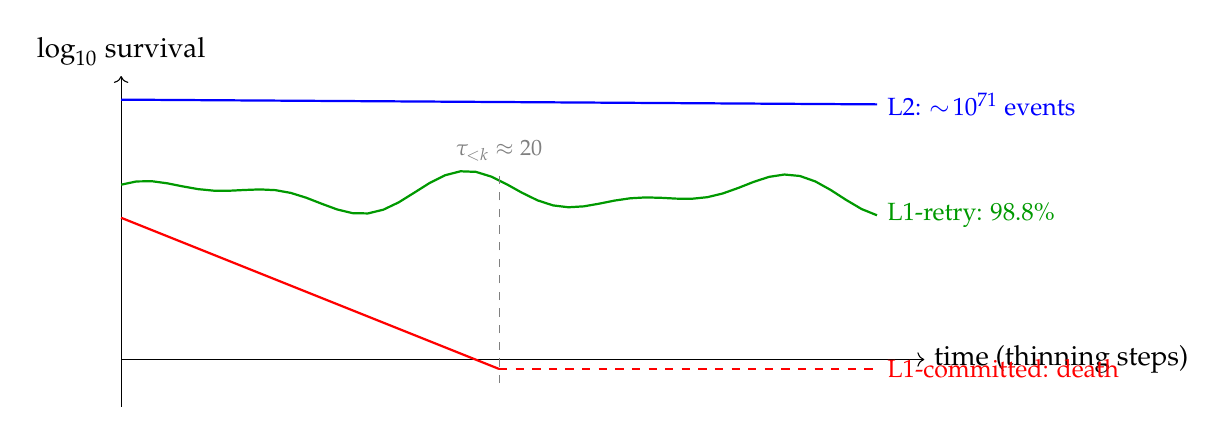
\begin{tikzpicture}[xscale=1.2, yscale=0.6]
  \draw[->] (0,0) -- (8.5,0) node[right] {time (thinning steps)};
  \draw[->] (0,-1) -- (0,6) node[above] {$\log_{10}$ survival};

  % L2 - nearly flat
  \draw[thick, blue] (0,5.5) -- (8,5.4)
    node[right, font=\small] {L2: $\sim\!10^{71}$ events};

  % L1-retry - fluctuating around 0.988
  \draw[thick, green!60!black, domain=0:8, samples=50]
    plot (\x, {3.5 + 0.3*sin(120*\x) + 0.2*cos(200*\x)})
    node[right, font=\small] {L1-retry: 98.8\%};

  % Committed - geometric decay
  \draw[thick, red, domain=0:4, samples=30]
    plot (\x, {3 - 0.8*\x})
    node[right, font=\small] {};
  \draw[thick, red, dashed, domain=4:8, samples=20]
    plot (\x, {-0.2}) node[right, font=\small] {L1-committed: death};

  % Death marker
  \draw[dashed, gray] (4,-0.5) -- (4,4) node[above, font=\footnotesize]
    {$\tau_{<k} \approx 20$};
\end{tikzpicture}
\caption{Survival dichotomy under compound streaming and thinning.
  Committed L1 dies in $O(\log d_0)$ steps.  L1-retry fluctuates at
  ${\sim}98.8\%$ stationarity.  L2 recurrence time is
  ${\sim}10^{71}$ events.}
\label{fig:survival}
\end{figure}

% ══════════════════════════════════════════════════════════════
\section{Empirical Validation}\label{sec:empirical}
% ══════════════════════════════════════════════════════════════

We summarize the empirical validation of the algebraic results.  Full
experimental details are in the companion papers
\cite{gaffney2026absorbing,gaffney2026streaming,gaffney2026mirage}.

\subsection{Absorbing-State Boundary}

The prefix-constraint impossibility theorem
(\cref{thm:prefix-impossibility}) was validated across $11{,}400$
boundary instances spanning $k = 0, \ldots, 5$ and $\varepsilon = 0.05,
\ldots, 0.95$ (100 seeds per configuration).  Under the
development-eligible counter $\jdev$:
\begin{itemize}[nosep]
  \item \textbf{False positives:} 0 (rule-of-three upper bound:
    $< 0.026\%$).
  \item \textbf{Trap rate:} 54.9\% across $4{,}200$ streaming instances
    (Wilson 95\% CI).
  \item \textbf{Recall:} 100\% ($0$ false negatives among $1{,}654$
    verified instances where $\min\text{-gap} < k$).
\end{itemize}
The non-hereditary structure (\cref{thm:non-hereditary}) was confirmed
on 40/40 tested instances with $n = 20$ events.

\begin{figure}[t]
\centering
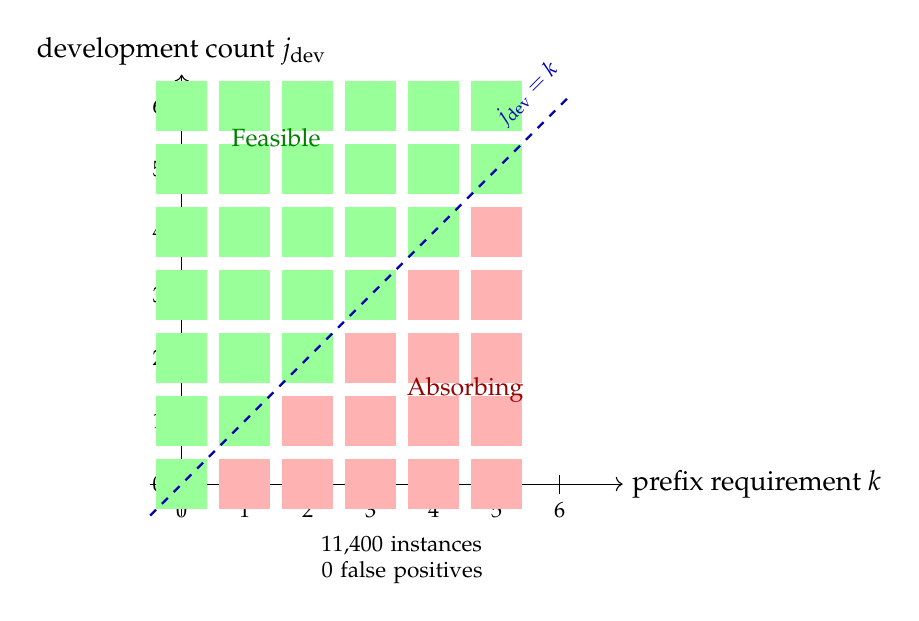
\begin{tikzpicture}[xscale=0.8, yscale=0.8]
  % Axes
  \draw[->] (-0.5,0) -- (7,0) node[right] {prefix requirement $k$};
  \draw[->] (0,-0.5) -- (0,6.5) node[above] {development count $\jdev$};

  % X-axis ticks
  \foreach \x in {0,...,6} {
    \draw (\x, -0.15) -- (\x, 0.15);
    \node[below=3pt, font=\footnotesize] at (\x, 0) {\x};
  }
  % Y-axis ticks
  \foreach \y in {0,...,6} {
    \draw (-0.15, \y) -- (0.15, \y);
    \node[left=3pt, font=\footnotesize] at (0, \y) {\y};
  }

  % Feasible region (j_dev >= k): green
  \foreach \k in {0,...,5} {
    \foreach \j in {0,...,6} {
      \pgfmathtruncatemacro{\feasible}{\j >= \k ? 1 : 0}
      \ifnum\feasible=1
        \fill[green!40] (\k-0.4, \j-0.4) rectangle (\k+0.4, \j+0.4);
      \fi
    }
  }

  % Infeasible region (j_dev < k): red
  \foreach \k in {1,...,5} {
    \foreach \j in {0,...,6} {
      \pgfmathtruncatemacro{\infeasible}{\j < \k ? 1 : 0}
      \ifnum\infeasible=1
        \fill[red!30] (\k-0.4, \j-0.4) rectangle (\k+0.4, \j+0.4);
      \fi
    }
  }

  % Boundary line (j_dev = k)
  \draw[thick, blue!70!black, dashed]
    (-0.5, -0.5) -- (6.2, 6.2);
  \node[blue!70!black, font=\footnotesize, rotate=45] at (5.5, 6.2)
    {$\jdev = k$};

  % Labels
  \node[font=\small, green!50!black] at (1.5, 5.5) {Feasible};
  \node[font=\small, red!60!black] at (4.5, 1.5) {Absorbing};

  % Zero FP annotation
  \node[font=\footnotesize, text width=3cm, align=center] at (3.5, -1.2)
    {$11{,}400$ instances\\0 false positives};
\end{tikzpicture}
\caption{Greedy validity boundary in the $(\jdev, k)$ plane.  Each
  cell represents a configuration tested across 100 seeds at
  $\varepsilon \in \{0.05, \ldots, 0.95\}$.  Green: feasible
  ($\jdev \ge k$).  Red: absorbed ($\jdev < k$).  The boundary
  $\jdev = k$ (dashed) is exact: zero false positives across $11{,}400$
  boundary instances.}
\label{fig:heatmap}
\end{figure}

\subsection{Algebraic Exactness}

The monoid structure (\cref{thm:absorbing-ideal}) was validated
empirically:
\begin{itemize}[nosep]
  \item \textbf{Pairwise composition:} 240 random pairs, 0 violations
    vs.\ event-level reference.
  \item \textbf{Absorbing-ideal closure:} 96 committed absorbing
    elements composed with random suffixes, 0 escapes.
  \item \textbf{Closure diagnostics:} Among elementary operations
    (composition, compression, pivot update, split), only compression
    violates closure (rate 0.133); all others have rate exactly~0.
\end{itemize}

\subsection{Turnover and the 4$\times$3 Matrix}

Turnover universality (\cref{thm:turnover}) holds in 103/103 observed
recovery events: every recovery is via $\argmax$ replacement, none via
same-pivot regrowth.

The complete survival matrix across four semantic models and three
algebraic levels (500 traces per cell, Wilson 95\% CIs) is:

\begin{table}[H]
\centering
\caption{Survival probability across semantic models and algebraic
  levels.  All entries from 500-trace simulations at canonical
  parameters ($r = 0.80$, $T = 100$, $p = 0.367$, $k = 3$).  Wilson
  95\% confidence intervals shown for L1-retry, the column with
  non-trivial variance; L1-absorb and L2 columns have near-degenerate
  distributions (all-or-nothing survival).}
\label{tab:4x3}
\begin{tabular}{@{}lccc@{}}
\toprule
\textbf{Model} & \textbf{L1-absorb} & \textbf{L1-retry (95\% CI)}
  & \textbf{L2} \\
\midrule
Fixed-focal      & 67.6\% & \textbf{98.2\%} (96.6--99.1\%) & \textbf{100.0\%} \\
Dynamic-focal    & 60.8\% & \textbf{98.8\%} (97.4--99.4\%) & 60.8\% \\
Protected-record & 0.2\%  & 20.6\% (17.3--24.4\%)          & 0.2\% \\
K-core           & 0.8\%  & 25.0\% (21.4--29.0\%)          & 0.8\% \\
\bottomrule
\end{tabular}
\end{table}

\noindent The table reveals two structural findings.  First, L1-retry
outperforms L2 under dynamic-focal semantics (98.8\% vs.\ 60.8\%),
inverting the algebraic hierarchy.  Second, pivot protection
(protected-record and K-core) is catastrophic under dynamic-focal
semantics: it destroys the $\argmax$ turnover mechanism that L1-retry
depends on.

\subsection{Turnover Universality}

\begin{table}[H]
\centering
\caption{Recovery mechanism in L1-retry under dynamic-focal semantics
  (103 recovery events observed).}
\label{tab:turnover}
\begin{tabular}{@{}lcc@{}}
\toprule
\textbf{Recovery mechanism} & \textbf{Count} & \textbf{Rate} \\
\midrule
New $\argmax$ (turnover)           & 103 & 100.0\% \\
Same $\argmax$ regains predecessors & 0   & 0.0\% \\
\bottomrule
\end{tabular}
\end{table}

% ══════════════════════════════════════════════════════════════
\section{Discussion}\label{sec:discussion}
% ══════════════════════════════════════════════════════════════

\subsection{Summary of Contributions}

This paper establishes the algebraic foundations of endogenous-pivot
semantics: a three-level tower (L1/L2/L3) with exact characterization
of the absorbing pathology, a tropical matrix equivalence enabling
parallel computation, a Myhill--Nerode optimality proof for L2, and a
record-gap spectrum placing streaming trap rates in the
Ewens$(\theta=1)$ universality class.  The dynamics under compression
are governed by three well-separated timescales: fast committed death,
stable L1-retry ergodicity, and astronomically slow L2 recurrence.
The operational retention floor (\cref{prop:retention-floor}) closes
the gap between the empirical regime boundary and the algebraic
framework, resolving what was an open problem at the outset of this
work.

\subsection{Related Work}

Our construction intersects several established literatures.

\paragraph{Tropical geometry and max-plus systems.}
The tropical matrix equivalence (\cref{thm:tropical-matrix}) embeds
our setting in the theory of max-plus linear algebra developed by
Baccelli~et~al.~\cite{baccelli1992synchronization}.  In classical
max-plus systems, the state matrices arise from deterministic timing
constraints---job durations, buffer capacities---and the spectral
theory of max-plus eigenvalues governs throughput and cycle times.  Our
matrices differ in that they encode \emph{semantic} composition: each
entry records a feasibility frontier across predecessor budgets, and the
matrix product implements the shift-and-max rule rather than a
scheduling recurrence.  As a consequence, the spectral properties of
our matrices are determined by the grammar parameter $k$ (the prefix
requirement) rather than by network topology.
Maclagan and Sturmfels~\cite{maclagan2015introduction} and
Joswig~\cite{joswig2021essentials} provide comprehensive treatments
of tropical geometry; our use is more algebraic than geometric, focused
on the monoid structure of $\Tmax^{(k+2)\times(k+2)}$ rather than on
tropical varieties or Newton polytopes.

\paragraph{Record theory and the CRP.}
The record-gap spectrum (\cref{thm:record-gap}) extends classical
record theory \cite{nevzorov2001records,arnold1998records} by
introducing the focal-mask model, which modifies the standard record
process via Bernoulli masking.  R\'enyi's foundational
work~\cite{renyi1962theorie} established the $1/g$ harmonic intensity
for i.i.d.\ records; our $\lambda_g(p) = [1-(1-p)^g]/g$ is the masked
generalization, recovering R\'enyi's result at $p \to 1$.  The Chinese
Restaurant Process coupling (\cref{thm:record-gap}, Step~E) connects
the gap spectrum to the Ewens$(\theta{=}1)$ sampling formula
\cite{ewens1972sampling}.  In the classical population genetics setting,
Ewens$(\theta)$ governs allele frequency spectra under neutral mutation;
our coupling maps gap sizes to table sizes via the integral
representation $\lambda_g = \int_0^a e^{-gy}\, dy$ with
$a = -\ln(1-p)$.  The truncation at $a < \infty$ (rather than the
$a = \infty$ used in the standard CRP) reflects the focal mask: a
fraction $1-p$ of events are invisible to the record process.  This
connection places the record-gap spectrum in the logarithmic
combinatorial structures framework of
Arratia--Barbour--Tavar\'e~\cite{arratia2003logarithmic}.

\paragraph{Automata theory and state lower bounds.}
The Myhill--Nerode necessity result (\cref{thm:myhill-nerode}) adapts
the classical automata-theoretic technique
\cite{hopcroft1979introduction} to algebraic summaries.  The standard
theorem establishes that the number of states in a minimal DFA equals
the number of equivalence classes of the syntactic right-congruence.
Our adaptation replaces the DFA by an associative summary algebra and
the acceptance predicate by feasibility at threshold~$k$.  The
resulting $\Omega(k)$ lower bound is tight (L2 achieves it), making L2
optimal among valid summaries (we conjecture it is, in fact, the
initial object in the category of valid summaries).
This contrasts with communication complexity lower bounds for
related problems (e.g., set disjointness, gap Hamming) where the lower
bound is typically information-theoretic.  Our bound is structural: it
counts the number of \emph{distinguishable futures} that a summary must
separate, and the separating suffixes have an explicit combinatorial
construction (\cref{ex:myhill-nerode-k3}).

\paragraph{Choice theory and path independence.}
The path-independence connection (\cref{app:plott}) links our
associativity result to Plott~\cite{plott1973path} and the
Moulin~\cite{moulin1985choice} classification of choice functions.
Plott's theorem establishes that single-valued path-independent choice
over a finite set is equivalent to $\argmax$ of a linear order---which
is precisely our pivot selection rule.  The
Danilov--Koshevoy~\cite{danilov2003choice} refinement clarifies
that this equivalence breaks for set-valued choice, a subtlety our
setting avoids via continuous weights (ensuring singleton selection
almost surely).  The algebraic consequence is that the endogenous
composition $\opendo$ is associative (\cref{thm:absorbing-ideal}(a)):
context elements can be composed in any order because the underlying
choice rule is path-independent.

\paragraph{Constrained generation and resource-constrained paths.}
Grammar-constrained decoding
\cite{scholak2021picard,willard2023efficient} enforces syntactic
constraints on LLM output via incremental parsing or finite-automaton
masking.  These approaches maintain an \emph{exogenous} constraint
state: the parse state depends only on the generated prefix, not on
future tokens.  The resource-constrained shortest path framework
\cite{irnich2005shortest} similarly maintains resource vectors that
evolve monotonically along the path.  Our endogenous pivot semantics
creates a qualitatively different constraint: the grammar's
interpretation depends on the output itself (specifically, on which
element is the $\argmax$), so the constraint state cannot be determined
incrementally from a prefix.  This is the fundamental reason that the
L2 tropical vector---which maintains the full feasibility frontier
across all possible pivot budgets---is necessary
(\cref{thm:myhill-nerode}) rather than merely convenient.

\subsection{Open Problems}

\begin{enumerate}[label=\arabic*.]
  \item \textbf{Complexity ceiling.}  The conjecture
    $k_{\max} = \lfloor 1/(4\sigma^2) \rfloor$ relating the maximum
    supportable prefix requirement to thinning variance awaits a
    rigorous mapping from $\sigma^2$ to the INAR parameters $(r, p, T)$.

  \item \textbf{Finite-$r$ dilogarithm correction.}  The
    Euler--Maclaurin approximation in \cref{thm:dilogarithm} introduces
    a ${\sim}1.4\%$ gap between $\mathrm{Li}_2(p)/p$ and the empirical
    scaling constant.  An $O(\varepsilon)$ correction term would close
    this.

  \item \textbf{Burstiness deformation.}  The focal-mask model assumes
    i.i.d.\ focal assignments.  A Nevzorov $F_\alpha$ deformation for
    front-loaded streams would extend \cref{thm:record-gap} to
    realistic bursty distributions.

  \item \textbf{Tight converse.}  \Cref{thm:turnover} proves committed
    death; \cref{prop:retention-floor} gives the fixed-focal floor
    $r^*(H,\delta)$.  A full converse---for any fixed horizon $H$, no
    strategy achieves survival probability $> 1 - \delta$ below
    $r^*(H,\delta)$---requires a matching lower bound showing that L2
    also fails at low retention.

  \item \textbf{Multi-agent coherence.}  A sheaf-cohomology
    decomposition of multi-agent extraction failure is conjectured, with
    $H^1$ encoding structural (combinatorial) obstructions and $H^2$
    encoding metric (weight-threshold) obstructions, but no computation
    exists.
\end{enumerate}

\subsection{Limitations}

The focal-mask model assumes i.i.d.\ focal events with continuous
weights, which may not hold in all applications.  The empirical
validation uses synthetic event graphs; real-world streams may exhibit
correlations not captured by the model.  The retention floor
(\cref{prop:retention-floor}) is derived under the i.i.d.\ assumption;
correlated focal weights or non-stationary thinning rates may shift
$r^*$ per domain.  The Myhill--Nerode argument assumes singleton
path-independent pivot selection; set-valued or non-path-independent
variants may require different state bounds.

% ══════════════════════════════════════════════════════════════
\section{Conclusion}\label{sec:conclusion}
% ══════════════════════════════════════════════════════════════

We have developed a complete algebraic theory for sequential extraction
under endogenous pivot semantics.  The core insight is that the
$\argmax$-selected pivot creates a circular dependence between the
selected set and its interpretation, placing the problem outside
classical greedy frameworks.  The three-level algebraic tower---scalar
monoid, tropical vector, frontier semiring---captures this pathology at
increasing levels of resolution, with the tropical vector (L2)
provably optimal via a Myhill--Nerode argument.

The tropical matrix equivalence connects our construction to the
well-studied theory of max-plus linear systems, and the record-gap
spectrum places streaming trap rates in the Ewens$(\theta=1)$
universality class---a surprising connection between endogenous
selection and combinatorial stochastic processes.

Under compound streaming and thinning, the system exhibits three
well-separated timescales: committed death is logarithmically fast,
L1-retry achieves near-perfect stationarity at $O(1)$ cost, and L2
recurrence involves the Euler dilogarithm and is operationally
infinite.  These results provide the algebraic foundation for designing
safe compression policies in systems with endogenous semantics.

% ══════════════════════════════════════════════════════════════
%  Bibliography
% ══════════════════════════════════════════════════════════════
\bibliographystyle{plainnat}
\bibliography{refs}

% ══════════════════════════════════════════════════════════════
%  Appendix
% ══════════════════════════════════════════════════════════════
\appendix

\section{Plott Path Independence Connection}
\label{app:plott}

The associativity of the endogenous composition $\opendo$ is intimately
related to Plott's path independence axiom \cite{plott1973path}; see
Moulin~\cite{moulin1985choice} for a comprehensive survey of choice
functions over finite sets.  Path independence requires:
\[
  \tau(A \cup \tau(B)) = \tau(A \cup B).
\]
Plott's theorem establishes that a single-valued path-independent choice
function over a finite set is equivalent to $\argmax$ of a strict linear
order.

In our setting, the endogenous pivot $\tau(S) = \argmax_{v \in S, a(v)
= a^*} w(v)$ is precisely such a function (assuming continuous weights
for almost-sure uniqueness).  The associativity of $\opendo$ is the
algebraic consequence: context elements can be composed in any order
because the pivot selection rule is path-independent.

The Danilov--Koshevoy refinement \cite{danilov2003choice} clarifies that
path independence alone does \emph{not} force $\argmax$ when the choice
function is set-valued.  The counterexample $\tau(S) = \{\min(S),
\max(S)\}$ is path-independent but not representable as $\argmax$ of a
single order.  Our setting avoids this subtlety because continuous
weights ensure singleton-valued selection.

\section{EIS Fiber Structure}\label{app:fibers}

The feasible family $\mathcal{F}$ decomposes into \textbf{fibers}
indexed by pivot identity: $\mathcal{F} = \bigcup_{p \in V} F_p$ where
$F_p = \{S \in \mathcal{F} : \tau(S) = p\}$.

Each fiber is an \emph{order filter} (upper set) in the Boolean lattice
of subsets: if $S \in F_p$ and $S \subseteq S'$ with $\tau(S') = p$,
then $S' \in F_p$ (adding events preserves feasibility when the pivot
is unchanged).  Fibers are \emph{not} matroids, since matroids require
downward closure (the hereditary axiom), while our fibers are upward
closed.

Three deletion operations characterize fiber boundaries:
\begin{enumerate}[nosep]
  \item \textbf{Post-pivot deletion:} pivot and $\dpre$ unchanged.
    Generally safe.
  \item \textbf{Pre-pivot non-focal deletion:} pivot unchanged but
    $\dpre$ decreases by 1.  Exits feasibility at the $\dpre = k$
    boundary.
  \item \textbf{Pivot deletion:} fiber transition to $F_{p'}$ where
    $p'$ is the next-heaviest focal event.  Structure changes entirely.
\end{enumerate}

\section{INAR(1) Stationary Distribution}\label{app:inar}

The INAR(1) process $N_{n+1} = \mathrm{Bin}(N_n, r) + \mathrm{Bin}(T,
pr)$ has a unique stationary distribution.  The probability generating
function satisfies:
\[
  G(z) = \mathbb{E}[z^{N_\infty}]
  = \prod_{m=0}^{\infty} (1 - pr^{m+1} + pr^{m+1} z)^T
  = \prod_{m=1}^{\infty} (1 - pr^m(1-z))^T.
\]
Setting $z = 0$:
\[
  \pi_0 = G(0) = \prod_{m=1}^{\infty} (1 - pr^m)^T,
\]
which is \cref{eq:pi0}.  The Kac mean return time is
$\mathbb{E}[\tau_0] = 1/\pi_0$.  At $r = 0.80$, $T = 100$,
$p = 0.367$: $\pi_0 \approx 1.3 \times 10^{-70}$, giving
$1/\pi_0 \approx 7.55 \times 10^{69}$ epochs $\approx 10^{71}$ events.

The scaling $\ln(1/\pi_0) \sim c \cdot \mu$ with
$c = \mathrm{Li}_2(p)/p$ follows from the Euler--Maclaurin analysis in
the proof of \cref{thm:dilogarithm}.

\subsection*{Lambert-series expansion and the retention floor}

The logarithm of the stationary zero probability admits a Lambert-series
expansion that clarifies both the moderate-$r$ and high-$r$ regimes of
\cref{prop:retention-floor}.

\begin{equation}\label{eq:lambert}
  \ln(1/\pi_0)
  = -T \sum_{m=1}^{\infty} \ln(1 - pr^m)
  = T \sum_{m=1}^{\infty} \sum_{s=1}^{\infty} \frac{(pr^m)^s}{s}
  = T \sum_{s=1}^{\infty} \frac{p^s}{s} \cdot \frac{r^s}{1 - r^s}.
\end{equation}
The last equality follows by exchanging the order of summation and
using $\sum_{m=1}^\infty r^{ms} = r^s/(1-r^s)$.

\paragraph{Term-by-term structure.}
Denote the $s$-th term $a_s = Tp^s r^s / [s(1-r^s)]$.  At canonical
parameters ($r = 0.80$, $T = 100$, $p = 0.367$):
\begin{center}
\begin{tabular}{@{}crrrr@{}}
\toprule
$s$ & $p^s$ & $r^s/(1-r^s)$ & $a_s$ & cumulative \\
\midrule
1 & $0.367$ & $4.000$ & $146.8$ & $146.8$ \\
2 & $0.135$ & $1.778$ & $12.0$ & $158.8$ \\
3 & $0.049$ & $1.047$ & $1.72$ & $160.5$ \\
4 & $0.018$ & $0.719$ & $0.33$ & $160.8$ \\
$\vdots$ & & & & \\
$\infty$ & & & & $161.1$ \\
\bottomrule
\end{tabular}
\end{center}
The $s = 1$ term alone captures $146.8/161.1 = 91.1\%$ of
$\ln(1/\pi_0)$.  The first four terms account for $99.8\%$.

\paragraph{Moderate-$r$ regime.}
When $r$ is small enough that $r^s \ll 1$ for $s \ge 2$, the $s = 1$
term dominates:
\[
  \ln(1/\pi_0) \approx a_1 = \frac{Tpr}{1-r} = \mu_f,
\]
the mean surviving focal count.  Setting $\mu_f = \ln H$ (from the
retention floor equation $\pi_0 = 1/H$ at $\delta \ll 1$) and
converting to non-focal buffer:
\[
  c(H) = \frac{\mu_{\mathrm{nf}}}{k}
  = \frac{(1-p)}{p} \cdot \frac{\mu_f}{k}
  \approx \frac{(1-p) \ln H}{pk}.
\]
This is exact to $O(p^2 r^2)$ relative error and does not require the
dilogarithm.

\paragraph{High-$r$ regime.}
As $r \to 1$, higher-order terms in \eqref{eq:lambert} become
significant.  The Euler--Maclaurin approximation replaces the sum over
$s$ by an integral:
\[
  \sum_{s=1}^{\infty} \frac{p^s}{s} \cdot \frac{r^s}{1-r^s}
  \approx \frac{1}{-\ln r}
  \sum_{s=1}^{\infty} \frac{p^s}{s^2}
  = \frac{\mathrm{Li}_2(p)}{-\ln r},
\]
where we used $r^s/(1-r^s) \approx 1/(s|\ln r|)$ for small
$|\ln r|$.  This gives $\ln(1/\pi_0) \approx T \cdot
\mathrm{Li}_2(p)/|\ln r| = \mathrm{Li}_2(p)/p \cdot \mu$, recovering
the dilogarithm scaling of \cref{thm:dilogarithm}.

\paragraph{Convergence at the fixed-focal floor.}
At $r^* \approx 0.304$ (the empirical fixed-focal retention floor),
the term ratios are: $a_2/a_1 = 0.033$, $a_3/a_1 = 0.0014$.  The
$s = 1$ approximation $\ln(1/\pi_0) \approx \mu_f$ is accurate to
$3.4\%$ at this retention rate, confirming that the moderate-$r$
formula in \cref{prop:retention-floor} applies.  At $r = 0.80$
(canonical), $a_2/a_1 = 0.082$ and the dilogarithm correction is
essential---the $s = 1$ term alone understates $\ln(1/\pi_0)$ by
$9.7\%$.

\end{document}
